\documentclass[twoside,11pt]{article}

\usepackage{graphicx}
\pagestyle{myheadings}

% +
%  Name:
%     sc11.tex
%
%  Purpose:
%     Mapping cookbook for SURF (SC/11)
%
%  Authors:
%     Tim Jenness (JAC)
%     Goeran Sandell (JAC/SOFIA)
%     Nick Jessop (JAC)
%
%  Copyright:
%     Copyright (C) 1997-2001 Particle Physics and Astronomy
%     Research Council. All Rights Reserved.
%
%  History:
%     1997-1998 (GS):
%        Original versions
%     Summer 2001 (GS/NEJ/TJ):
%        Updates to keep in line with new KAPPA and SURF
%        Add SCAN MAP information
%        Rewrite calibration section
%        Add new authors
%     13 October 2001 (GS):
%        Final updates
%     29 October 2001 (TJ):
%        Integrate back into SURF distribution
%     {Add further history here}
%
% -

% ------------------------------------------------------------------------


% Add any \newcommand or \newenvironment commands here
\newcommand{\about}{$\sim$}
\newcommand{\eg}{{\it e.g.}}
\newcommand{\ie}{{\it i.e.}}
\newcommand{\mic}{\mbox{\,${\mu}$m}}               % microns
\newcommand{\arcmin}{{$^\prime$}}
\newcommand{\degr}{\mbox{\,$^\circ$}}               % degrees sign
% ------------------------------------------------------------------------



% ------------------------------------------------------------------------


% ? Document identification
\newcommand{\stardoccategory}  {Starlink Cookbook}
\newcommand{\stardocinitials}  {SC}
\newcommand{\stardocsource}    {sc\stardocnumber}
\newcommand{\stardocnumber}    {11.2}
\newcommand{\stardocauthors}   {G. Sandell, N. Jessop, T. Jenness \\
Joint Astronomy Centre, Hilo, Hawaii}
\newcommand{\stardocdate}      {29th October 2001}
\newcommand{\stardoctitle}     {The SCUBA map reduction cookbook}
\newcommand{\stardocversion}   {\ }
\newcommand{\stardocmanual}    {\ }
\newcommand{\stardocabstract}  {[Text of abstract]}
% ? End of document identification

% A new environment for quoting verbatim
% Environment for indenting and using a small font.
\newenvironment{myquote}{\begin{quote}\begin{small}}{\end{small}\end{quote}}



\newcommand{\text}[1]{{\small \texttt{#1}}}

% SCUBA reference
\newcommand{\scuba}{\htmladdnormallink{SCUBA}{http://www.jach.hawaii.edu/JCMT/}}


% Starlink Package names
\newcommand{\starlink}{\htmladdnormallink{Starlink}{http://www.starlink.ac.uk/}}


% set up some common package names
\newcommand{\Kappa}{\xref{\textsc{Kappa}}{sun95}{}}
\newcommand{\Figaro}{\xref{\textsc{Figaro}}{sun86}{}}
\newcommand{\gaia}{\xref{\textsc{Gaia}}{sun214}{}}
\newcommand{\convert}{\xref{\textsc{Convert}}{sun55}{}}
\newcommand{\fluxes}{\xref{\textsc{Fluxes}}{sun213}{}}
\newcommand{\ccdpack}{\xref{\textsc{Ccdpack}}{sun139}{}}
\newcommand{\Iras}{\xref{\textsc{Iras90}}{sun163}{}}
\newcommand{\ndf}{\xref{NDF}{sun33}{}}
\newcommand{\agi}{\xref{AGI}{sun48}{}}
\newcommand{\surf}{\xref{\textsc{Surf}}{sun216}{}}
\newcommand{\Specdre}{\xref{\textsc{Specdre}}{sun140}{}}
\newcommand{\jcmtdr}{\xref{\textsc{JCMTdr}}{sun132}{}}
\newcommand{\nod}{\textsc{nod2}}
\newcommand{\ESP}{\xref{ESP}{sun180}{}}
\newcommand{\GKS}{\xref{GKS}{sun83}{}}
\newcommand{\oracdr}{\xref{\textsc{orac-dr}}{sun231}{}}

% Application tasks
\newcommand{\task}[1]{\textsf{#1}}

% ADAM parameters
\newcommand{\param}[1]{\texttt{#1}}

% SURF tasks
\newcommand{\rebin}{\xref{\task{rebin}}{sun216}{REBIN}}
\newcommand{\remdbm}{\xref{\task{remdbm}}{sun216}{REMDBM}}
\newcommand{\bolrebin}{\xref{\task{bolrebin}}{sun216}{BOLREBIN}}
\newcommand{\intrebin}{\xref{\task{intrebin}}{sun216}{INTREBIN}}
\newcommand{\calcsky}{\xref{\task{calcsky}}{sun216}{CALCSKY}}
\newcommand{\chgqual}{\xref{\task{change\_\-qua\-lity}}{sun216}{CHANGE_QUALITY}}


\newcommand{\chgflat}{\xref{\task{change\_flat}}{sun216}{CHANGE_FLAT}}
\newcommand{\chgpnt}{\xref{\task{change\_pointing}}{sun216}{CHANGE_POINTING}}


\newcommand{\chgdata}{\xref{\task{change\_data}}{sun216}{CHANGE_DATA}}
\newcommand{\desp}{\xref{\task{despike}}{sun216}{DESPIKE}}
%\newcommand{\desp2}{\xref{\task{despike2}}{sun216}{DESPIKE2}}
\newcommand{\dspbol}{\xref{\task{dspbol}}{sun216}{DSPBOL}}
\newcommand{\resw}{\xref{\task{reduce\_switch}}{sun216}{REDUCE_SWITCH}}


\newcommand{\flatf}{\xref{\task{flatfield}}{sun216}{FLATFIELD}}
\newcommand{\skydip}{\xref{\task{skydip}}{sun216}{SKYDIP}}

\newcommand{\scuphot}{\xref{\task{scuphot}}{sun216}{SCUPHOT}}
\newcommand{\scanrlb}{\xref{\task{scan\_rlb}}{sun216}{SCAN_RLB}}
\newcommand{\ext}{\xref{\task{extinction}}{sun216}{EXTINCTION}}
\newcommand{\scuquick}{\xref{\task{scuquick}}{sun216}{SCUQUICK}}
\newcommand{\scuhelp}{\xref{\task{scuhelp}}{sun216}{SCUHELP}}
\newcommand{\remsky}{\xref{\task{remsky}}{sun216}{REMSKY}}
\newcommand{\scuover}{\xref{\task{scuover}}{sun216}{SCUOVER}}
\newcommand{\extdata}{\xref{\task{extract\_data}}{sun216}{EXTRACT_DATA}}


\newcommand{\sculog}{\xref{\task{sculog}}{sun216}{SCULOG}}
\newcommand{\scuplot}{\xref{\task{scuplot}}{sun216}{SCUPLOT}}
\newcommand{\scucat}{\xref{\task{scucat}}{sun216}{SCUCAT}}
\newcommand{\photsum}{\xref{\task{photsum}}{sun216}{PHOTSUM}}
\newcommand{\mapsum}{\xref{\task{mapsum}}{sun216}{MAPSUM}}
\newcommand{\pointsum}{\xref{\task{pointsum}}{sun216}{POINTSUM}}
\newcommand{\qdraw}{\xref{\task{qdraw}}{sun216}{QDRAW}}
\newcommand{\sigclip}{\xref{\task{sigclip}}{sun216}{SIGCLIP}}
\newcommand{\restore}{\xref{\task{restore}}{sun216}{RESTORE}}
\newcommand{\sdip}{\xref{\task{sdip}}{sun216}{SDIP}}
\newcommand{\scuclip}{\xref{\task{scuclip}}{sun216}{SCUCLIP}}
\newcommand{\scupa}{\xref{\task{scupa}}{sun216}{SCUPA}}
\newcommand{\scunoise}{\xref{\task{scunoise}}{sun216}{SCUNOISE}}
\newcommand{\obssum}{\xref{\task{obssum}}{sun216}{OBSSUM}}

% Non surf tasks

% KAPPA
\newcommand{\display}{\xref{\task{display}}{sun95}{DISPLAY}}
\newcommand{\aperadd}{\xref{\task{aperadd}}{sun95}{APERADD}}
\newcommand{\linplot}{\xref{\task{linplot}}{sun95}{LINPLOT}}
\newcommand{\mlinplot}{\xref{\task{mlinplot}}{sun95}{MLINPLOT}}
\newcommand{\drawsig}{\xref{\task{drawsig}}{sun95}{DRAWSIG}}
\newcommand{\centroid}{\xref{\task{centroid}}{sun95}{CENTROID}}
\newcommand{\hislist}{\xref{\task{hislist}}{sun95}{HISLIST}}
\newcommand{\globals}{\xref{\task{globals}}{sun95}{GLOBALS}}
\newcommand{\setaxis}{\xref{\task{setaxis}}{sun95}{SETAXIS}}
\newcommand{\kstest}{\xref{\task{kstest}}{sun95}{KSTEST}}
\newcommand{\stats}{\xref{\task{stats}}{sun95}{STATS}}
\newcommand{\thresh}{\xref{\task{thresh}}{sun95}{THRESH}}
\newcommand{\setbb}{\xref{\task{setbb}}{sun95}{SETBB}}

\newcommand{\fitslist}{\xref{\task{fitslist}}{sun95}{FITSLIST}}
\newcommand{\fitsedit}{\xref{\task{fitsedit}}{sun95}{FITSEDIT}}

\newcommand{\setvar}{\xref{\task{setvar}}{sun95}{SETVAR}}
\newcommand{\ndfcopy}{\xref{\task{ndfcopy}}{sun95}{NDFCOPY}}
\newcommand{\gdset}{\xref{\task{gdset}}{sun95}{GDSET}}
\newcommand{\idset}{\xref{\task{idset}}{sun95}{IDSET}}
\newcommand{\ovset}{\xref{\task{ovset}}{sun95}{OVSET}}
\newcommand{\gdnames}{\xref{\task{gdnames}}{sun95}{GDNAMES}}
\newcommand{\gdclear}{\xref{\task{gdclear}}{sun95}{GDCLEAR}}
\newcommand{\cursor}{\xref{\task{cursor}}{sun95}{CURSOR}}
\newcommand{\flip}{\xref{\task{flip}}{sun95}{FLIP}}
\newcommand{\cadd}{\xref{\task{cadd}}{sun95}{CADD}}

\newcommand{\cdiv}{\xref{\task{cdiv}}{sun95}{CDIV}}
\newcommand{\Div}{\xref{\task{div}}{sun95}{DIV}}
\newcommand{\cmult}{\xref{\task{cmult}}{sun95}{CMULT}}
\newcommand{\mult}{\xref{\task{mult}}{sun95}{MULT}}
\newcommand{\add}{\xref{\task{add}}{sun95}{ADD}}
\newcommand{\sub}{\xref{\task{sub}}{sun95}{SUB}}
\newcommand{\csub}{\xref{\task{csub}}{sun95}{CSUB}}
\newcommand{\psf}{\xref{\task{psf}}{sun95}{PSF}}

\newcommand{\glitch}{\xref{\task{glitch}}{sun95}{GLITCH}}
\newcommand{\setunits}{\xref{\task{setunits}}{sun95}{SETUNITS}}
\newcommand{\fitstext}{\xref{\task{fitstext}}{sun95}{FITSTEXT}}
\newcommand{\fitsmod}{\xref{\task{fitsmod}}{sun95}{FITSMOD}}
\newcommand{\fitshead}{\xref{\task{fitshead}}{sun95}{FITSHEAD}}
\newcommand{\lutbgyrw}{\xref{\task{lutbgyrw}}{sun95}{LUTBGYRW}}
\newcommand{\contour}{\xref{\task{contour}}{sun95}{CONTOUR}}
\newcommand{\contover}{\xref{\task{contover}}{sun95}{CONTOVER}}

\newcommand{\turbocont}{\xref{\task{turbocont}}{sun95}{TURBOCONT}}
\newcommand{\mosaic}{\xref{\task{mosaic}}{sun95}{MOSAIC}}
\newcommand{\pixdupe}{\xref{\task{pixdupe}}{sun95}{PIXDUPE}}
\newcommand{\rotate}{\xref{\task{rotate}}{sun95}{ROTATE}}
\newcommand{\setbound}{\xref{\task{setbound}}{sun95}{SETBOUND}}
\newcommand{\slide}{\xref{\task{slide}}{sun95}{SLIDE}}
\newcommand{\gausmooth}{\xref{\task{gausmooth}}{sun95}{GAUSMOOTH}}
\newcommand{\median}{\xref{\task{median}}{sun95}{MEDIAN}}

\newcommand{\memd}{\xref{\task{mem2d}}{sun95}{MEM2D}}
\newcommand{\axlabel}{\xref{\task{axlabel}}{sun95}{AXLABEL}}
\newcommand{\axunits}{\xref{\task{axunits}}{sun95}{AXUNITS}}
\newcommand{\setlabel}{\xref{\task{setlabel}}{sun95}{SETLABEL}}
\newcommand{\settitle}{\xref{\task{settitle}}{sun95}{SETTITLE}}
\newcommand{\histogram}{\xref{\task{histogram}}{sun95}{HISTOGRAM}}
\newcommand{\normalize}{\xref{\task{normalize}}{sun95}{NORMALIZE}}

% Convert
\newcommand{\ndffits}{\xref{\task{ndf2fits}}{sun55}{NDF2FITS}}
\newcommand{\ndfascii}{\xref{\task{ndf2ascii}}{sun55}{NDF2ASCII}}

% FIGARO
\newcommand{\wdfits}{\xref{\task{wdfits}}{sun86}{WDFITS}}
\newcommand{\istat}{\xref{\task{istat}}{sun86}{ISTAT}}
\newcommand{\delobj}{\xref{\task{delobj}}{sun86}{DELOBJ}}
\newcommand{\copobj}{\xref{\task{copobj}}{sun86}{COPOBJ}}
\newcommand{\image}{\xref{\task{image}}{sun86}{IMAGE}}
\newcommand{\bclean}{\xref{\task{bclean}}{sun86}{BCLEAN}}
\newcommand{\ystract}{\xref{\task{ystract}}{sun86}{YSTRACT}}
\newcommand{\sclean}{\xref{\task{sclean}}{sun86}{SCLEAN}}

% CCDPACK
\newcommand{\makemos}{\xref{\task{makemos}}{sun139}{MAKEMOS}}

% IRAS90
\newcommand{\skypos}{\xref{\task{skypos}}{sun163}{SKYPOS}}
\newcommand{\skygrid}{\xref{\task{skygrid}}{sun163}{SKYGRID}}
\newcommand{\skyphot}{\xref{\task{skyphot}}{sun163}{SKYPHOT}}


% Misc
\newcommand{\hdstrace}{\xref{\task{hdstrace}}{sun102}{}}
\newcommand{\psmerge}{\xref{\task{psmerge}}{sun164}{}}
\newcommand{\fitgauss}{\xref{\task{fitgauss}}{sun140}{FITGAUSS}}
\newcommand{\gaufit}{\xref{\task{gaufit}}{sun180}{GAUFIT}}

% JAC

\newcommand{\Archibald}{\htmladdnormallink{Archibald}{http://www.jach.hawaii.edu/JACdocs/JCMT/SCD/SN/002.2/ } }
\newcommand{\Coulson}{\htmladdnormallink{Coulson}{http://www.jach.hawaii.edu/JACdocs/JCMT/SCD/SN/003/ }}


% +
%  Name:
%     sc.tex
%
%  Purpose:
%     Template for Starlink Cookbook (SC) documents.
%     Refer to SUN/199
%
%  Authors:
%     AJC: A.J.Chipperfield (Starlink, RAL)
%     BLY: M.J.Bly (Starlink, RAL)
%     PWD: Peter W. Draper (Starlink, Durham University)
%
%  History:
%     16-JUN-1997 (BLY):
%        Original, based on SUN/SG templates.
%     13-AUG-1998 (PWD):
%        Converted for use with LaTeX2HTML version 98.2 and
%        Star2HTML version 1.3.
%     {Add further history here}
%
% -

\newcommand{\stardocname}{\stardocinitials /\stardocnumber}
\markboth{\stardocname}{\stardocname}
\setlength{\textwidth}{160mm}
\setlength{\textheight}{230mm}
\setlength{\topmargin}{-2mm}
\setlength{\oddsidemargin}{0mm}
\setlength{\evensidemargin}{0mm}
\setlength{\parindent}{0mm}
\setlength{\parskip}{\medskipamount}
\setlength{\unitlength}{1mm}

% -------------------------------------------------------------------------


%  Hypertext definitions.
%  ======================
% These are used by the LaTeX2HTML translator in conjunction with
% star2html.

%  Comment.sty: version 2.0, 19 June 1992
%  Selectively in/exclude pieces of text.
%
%  Author
%    Victor Eijkhout
%    <eijkhout@cs.utk.edu>
%    Department of Computer Science
%    University Tennessee at Knoxville
%    104 Ayres Hall
%    Knoxville, TN 37996
%    USA

%  Do not remove the %begin{latexonly} and %end{latexonly} lines (used by
%  LaTeX2HTML to signify text it shouldn't process).
%begin{latexonly}
\makeatletter
\def\makeinnocent#1{\catcode`#1=12 }
\def\csarg#1#2{\expandafter#1\csname#2\endcsname}

\def\ThrowAwayComment#1{\begingroup
    \def\CurrentComment{#1}%
    \let\do\makeinnocent \dospecials
    \makeinnocent\^^L% and whatever other special cases
    \endlinechar`\^^M \catcode`\^^M=12 \xComment}
{\catcode`\^^M=12 \endlinechar=-1 %
 \gdef\xComment#1^^M{\def\test{#1}
      \csarg\ifx{PlainEnd\CurrentComment Test}\test
          \let\html@next\endgroup
      \else \csarg\ifx{LaLaEnd\CurrentComment Test}\test
            \edef\html@next{\endgroup\noexpand\end{\CurrentComment}}
      \else \let\html@next\xComment
      \fi \fi \html@next}
}
\makeatother

\def\includecomment
 #1{\expandafter\def\csname#1\endcsname{}%
    \expandafter\def\csname end#1\endcsname{}}
\def\excludecomment
 #1{\expandafter\def\csname#1\endcsname{\ThrowAwayComment{#1}}%
    {\escapechar=-1\relax
     \csarg\xdef{PlainEnd#1Test}{\string\\end#1}%
     \csarg\xdef{LaLaEnd#1Test}{\string\\end\string\{#1\string\}}%
    }}

%  Define environments that ignore their contents.
\excludecomment{comment}
\excludecomment{rawhtml}
\excludecomment{htmlonly}

%  Hypertext commands etc. This is a condensed version of the html.sty
%  file supplied with LaTeX2HTML by: Nikos Drakos
%  <nikos@cbl.leeds.ac.uk> &
%  Jelle van Zeijl <jvzeijl@isou17.estec.esa.nl>. The LaTeX2HTML
%  documentation
%  should be consulted about all commands (and the environments
%  defined above)
%  except \xref and \xlabel which are Starlink specific.

\newcommand{\htmladdnormallinkfoot}[2]{#1\footnote{#2}}
\newcommand{\htmladdnormallink}[2]{#1}
\newcommand{\htmladdimg}[1]{}
\newcommand{\hyperref}[4]{#2\ref{#4}#3}
\newcommand{\htmlref}[2]{#1}
\newcommand{\htmlimage}[1]{}
\newcommand{\htmladdtonavigation}[1]{}

\newenvironment{latexonly}{}{}
\newcommand{\latex}[1]{#1}
\newcommand{\html}[1]{}
\newcommand{\latexhtml}[2]{#1}
\newcommand{\HTMLcode}[2][]{}

%  Starlink cross-references and labels.
\newcommand{\xref}[3]{#1}
\newcommand{\xlabel}[1]{}

%  LaTeX2HTML symbol.
\newcommand{\latextohtml}{\LaTeX2\texttt{HTML}}

%  Define command to re-centre underscore for Latex and leave as normal
%  for HTML (severe problems with \_ in tabbing environments and \_\_
%  generally otherwise).
\renewcommand{\_}{\texttt{\symbol{95}}}

% ------------------------------------------------------------------------


%  Debugging.
%  =========
%  Remove % on the following to debug links in the HTML version using
%  Latex.

% \newcommand{\hotlink}[2]{\fbox{\begin{tabular}[t]{@{}c@{}}#1\\\hline{\footnotesize #2}\end{tabular}}}
% \renewcommand{\htmladdnormallinkfoot}[2]{\hotlink{#1}{#2}}
% \renewcommand{\htmladdnormallink}[2]{\hotlink{#1}{#2}}
% \renewcommand{\hyperref}[4]{\hotlink{#1}{\S\ref{#4}}}
% \renewcommand{\htmlref}[2]{\hotlink{#1}{\S\ref{#2}}}
% \renewcommand{\xref}[3]{\hotlink{#1}{#2 -- #3}}
%end{latexonly}
% -------------------------------------------------------------------------


% ? Document specific \newcommand or \newenvironment commands.
% ? End of document specific commands
% -------------------------------------------------------------------------


%  Title Page.
%  ===========
\renewcommand{\thepage}{\roman{page}}
\begin{document}
\thispagestyle{empty}

%  Latex document header.
%  ======================
\begin{latexonly}
   CCLRC / {\textsc Rutherford Appleton Laboratory} \hfill {\textbf
\stardocname}\\
   {\large Particle Physics \& Astronomy Research Council}\\
   {\large Starlink Project\\}
   {\large \stardoccategory\ \stardocnumber}
   \begin{flushright}
   \stardocauthors\\
   \stardocdate
   \end{flushright}
   \vspace{-4mm}
   \rule{\textwidth}{0.5mm}
   \vspace{5mm}
   \begin{center}
   {\Huge\textbf  \stardoctitle \\ [2.5ex]}
   {\LARGE\textbf \stardocversion \\ [4ex]}
   {\Huge\textbf  \stardocmanual}
   \end{center}
%   \vspace{5mm}

% ? Add picture here if required for the LaTeX version.
%   e.g. \includegraphics[scale=0.3]{filename.ps}
\begin{center}

\includegraphics[width=2.0in]{sc11_logo}
\end{center}
% ? End of picture

% ? Heading for abstract if used.
%   \vspace{10mm}
%   \begin{center}
%      {\Large\textbf Abstract}
%   \end{center}
% ? End of heading for abstract.
\end{latexonly}

%  HTML documentation header.
%  ==========================
\begin{htmlonly}
   \xlabel{}
   \begin{rawhtml} <H1 ALIGN=CENTER> \end{rawhtml}
      \stardoctitle\\
      \stardocversion\\
      \stardocmanual
   \begin{rawhtml} </H1> <HR> \end{rawhtml}

% ? Add picture here if required for the hypertext version.
%   e.g. \includegraphics[scale=0.7]{filename.ps}

\includegraphics[width=2.0in]{sc11_logo}
% ? End of picture

   \begin{rawhtml} <P> <I> \end{rawhtml}
   \stardoccategory\ \stardocnumber \\
   \stardocauthors \\
   \stardocdate
   \begin{rawhtml} </I> </P> <H3> \end{rawhtml}
      \htmladdnormallink{CCLRC}{http://www.cclrc.ac.uk} /
      \htmladdnormallink{Rutherford Appleton Laboratory}
                        {http://www.cclrc.ac.uk/ral} \\
      \htmladdnormallink{Particle Physics \& Astronomy Research
Council}
                        {http://www.pparc.ac.uk} \\
   \begin{rawhtml} </H3> <H2> \end{rawhtml}
      \htmladdnormallink{Starlink Project}{http://www.starlink.ac.uk/}
   \begin{rawhtml} </H2> \end{rawhtml}
   \htmladdnormallink{\htmladdimg{source.gif} Retrieve hardcopy}
      {http://www.starlink.ac.uk/cgi-bin/hcserver?\stardocsource}\\

%  HTML document table of contents.
%  ================================
%  Add table of contents header and a navigation button to return to
%  this point in the document (this should always go before the
%  abstract \section).
  \label{stardoccontents}
  \begin{rawhtml}
    <HR>
    <H2>Contents</H2>
  \end{rawhtml}
  \htmladdtonavigation{\htmlref{\htmladdimg{contents_motif.gif}}
        {stardoccontents}}

% ? New section for abstract if used.
%  \section{\xlabel{abstract}Abstract}
% ? End of new section for abstract
\end{htmlonly}

% ------------------------------------------------------------------------


% ? Document Abstract. (if used)
%  ==================
%\stardocabstract
% ? End of document abstract
% ------------------------------------------------------------------------


% ? Latex document Table of Contents (if used).
%  ===========================================
  \newpage
  \begin{latexonly}
    \setlength{\parskip}{0mm}
    \tableofcontents
    \setlength{\parskip}{\medskipamount}
    \markboth{\stardocname}{\stardocname}
  \end{latexonly}
% ? End of Latex document table of contents
% -------------------------------------------------------------------------


\cleardoublepage
\renewcommand{\thepage}{\arabic{page}}
\setcounter{page}{1}


\section{\xlabel{introduction}Introduction}

This is the revised guide on how to reduce, and analyze maps obtained
with \scuba\ using the off line SCUBA reduction package \surf\
\cite{surf} and the \starlink\ versions of \Kappa \cite{kappa},
\Figaro \cite{figaro}, \gaia \cite{gaia}, and \convert \cite{convert}.


The easiest way of using these packages is to run-up \oracdr, a
general purpose pipeline for reducing data from any telescope.  A set
of data reduction recipes are available to \oracdr\ for use when
working with scuba maps, these recipes utilize the \surf and \Kappa\ packages.


This cookbook makes no attempts to explain why and how, for that there
is a comprehensive Starlink User Note
(\xref{\textbf{SUN/216}}{sun216}{}) written by T. Jenness and J.
Lightfoot, which properly documents all the software tasks in \surf,
which should be consulted for those who need to know details of a
task, or how the task really works.


\section{\xlabel{The really easy way}The really easy way}

Given that \oracdr\ is what you will use at the telescope, and that it
provides the easiest introduction to the various steps necessary to
reduce your data, we will deal with it first. If you are at the
telescope log into \texttt{mamo} (if you are working on another machine just
\texttt{ssh mamo}), and then type:

\begin{myquote}
\begin{verbatim}
% oracdr_scuba
% oracdr
\end{verbatim}
\end{myquote}

\begin{figure}
\begin{center}
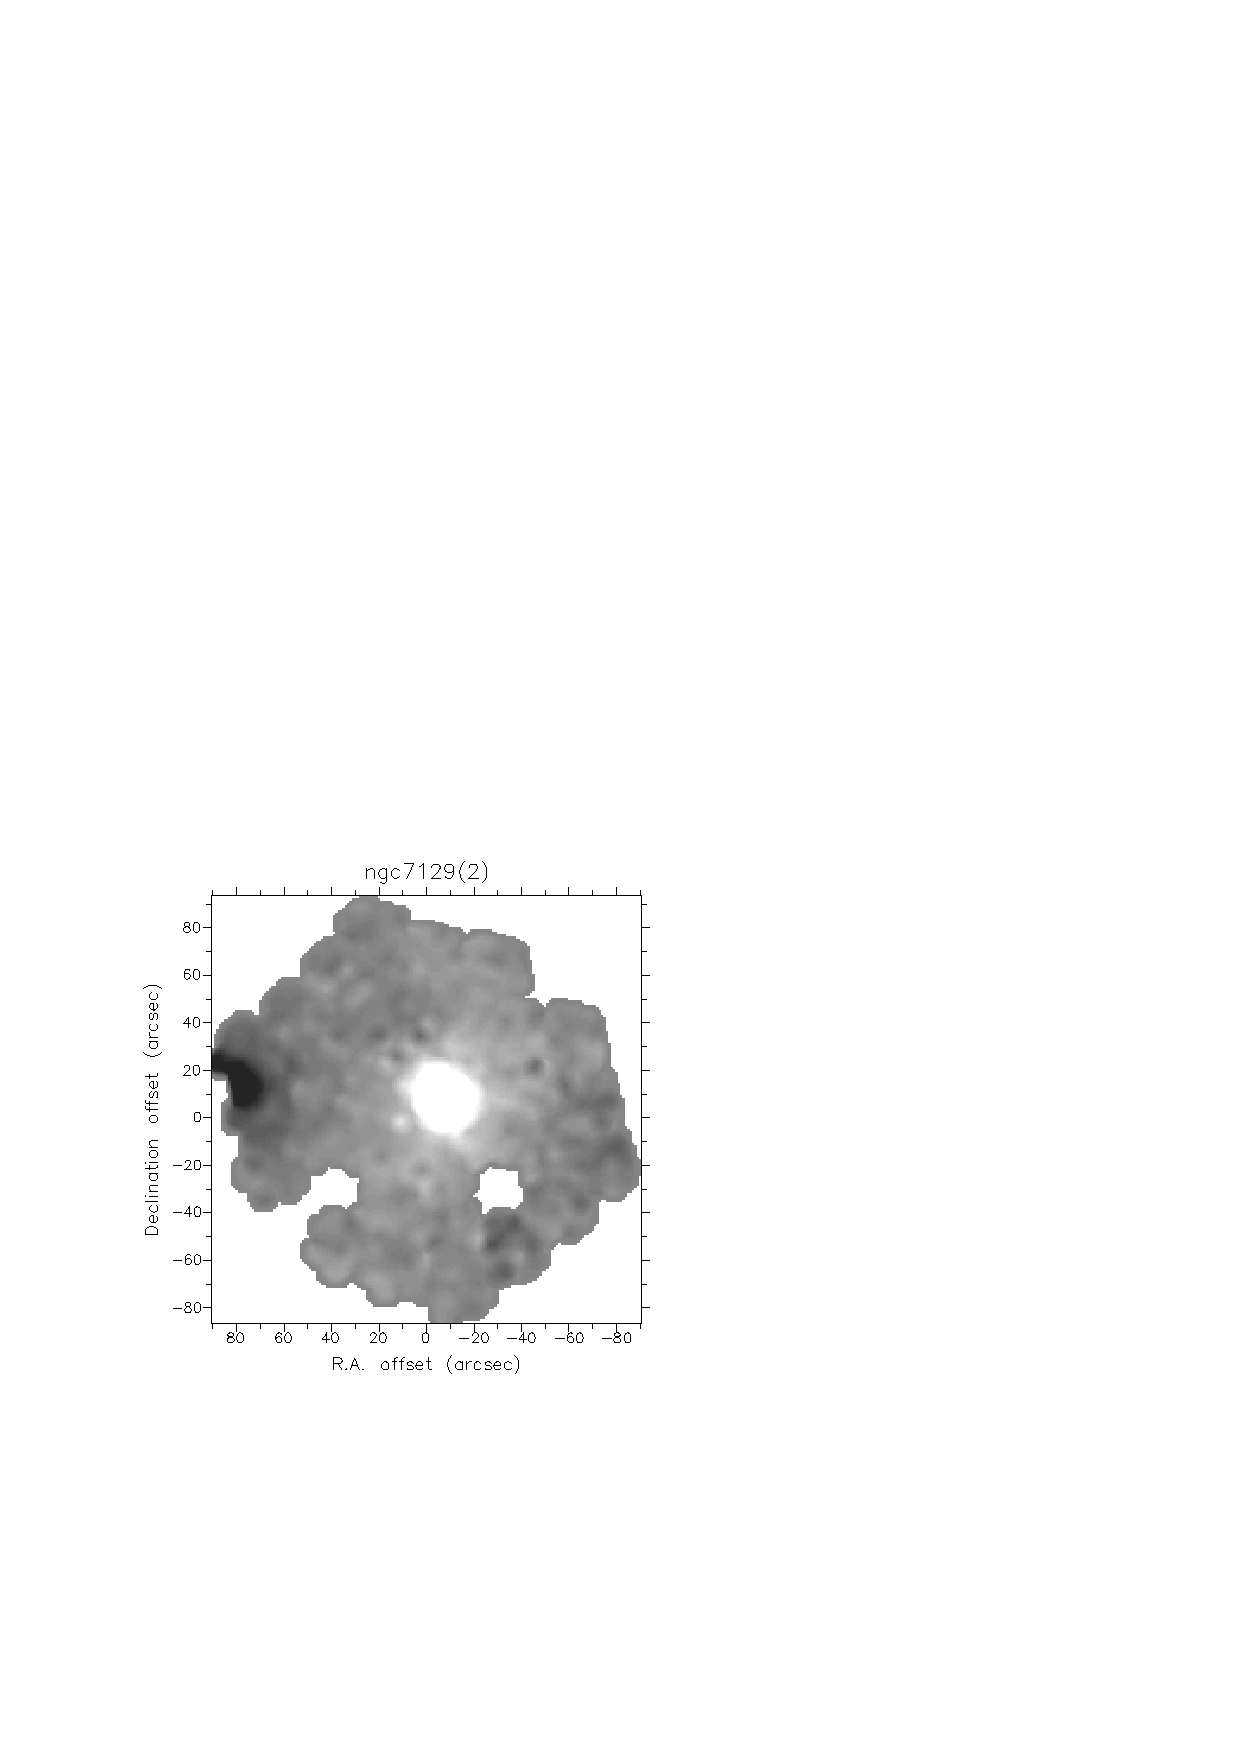
\includegraphics[width=5.5in]{sc11_fig1}
\caption{The \texttt{Xoracdr} gui for \textsc{orac-dr}.
  All the information needed to start
  the data reduction (ie. where the data is, what instrument is being used,
  what ut date) is prompted for.}
\label{fig:xoracdr}
\end{center}
\end{figure}

If you are at your home institution or at the JAC, you should use the
new x-windows gui. Simply type:

\begin{myquote}
\begin{verbatim}
%xoracdr
\end{verbatim}
\end{myquote}

and the interface shown in Figure \ \ref{fig:xoracdr} should pop-up.
Fill in the appropriate date, the location of the raw data files (see
below if you are at the JAC and unsure) as well as where you want the
reduced data to go, and press Start!

Having done one or other of the previous set-ups you should then find
a dialogue window pops up, with explanatory messages about what the
pipeline is doing, followed shortly by a xwindow which will display
all the key stages of the reduction.  You will find that \oracdr\
starts working through the observations one by one ignoring some (like
the focus and align measurements) but reducing most.  For each
distinct type of observation (pointing, skydip, jigglemap) \oracdr\
has a recipe it uses to reduce the data.  If you miss a stage (maybe
you went out to make a coffee) or you want to examine something in
detail, don't despair look at the output directory for the reduction,
you will find many of the final reduced files and intermediate stages
eating into your disk space.  From the name of the file you should be
able to work out at what stage of the reduction it was produced -- the
final `re-binned images' should finish in ``\texttt{\_reb}''.

Given this is a cookbook for reducing map data, let's look at the two
recipes for reducing jiggle-maps, and emerson2 maps.  You can find
these by typing ``\texttt{ls \$ORAC\_DIR/recipes/SCUBA}'' (if the environment
variable is not set type ``\texttt{oracdr\_scuba}'').  The jiggle map recipe
reads,

\begin{myquote}
\begin{verbatim}

=head1 NAME

SCUBA_JIGMAP - Standard reduction for jiggle map data

=head1 SYNOPSIS


=head1 DESCRIPTION

This is the standard recipe to use for reduction of SCUBA
jiggle map data.


=cut

_PRE_PROCESS_

_FLAT_FIELD_

_SET_BAD_PIXELS_

_EXTINCTION_CORRECT_

_CLIP_BOLOMETERS_ NSIGMA=5.0

_REMOVE_SKY_NOISE_JIGGLE_  BOLOMETERS=r3 MODE=median

_REBIN_FRAME_ PIXEL_SIZE=3.0 REBIN_METHOD=GAUSSIAN

_FIND_CALIBRATION_MAP_

_CALIBRATE_DATA_

_REBIN_GROUP_ PIXEL_SIZE=1.0 REBIN_METHOD=LINEAR

_DELETE_TEMP_FILES_ KEEP=_reb,_ext,_sky,_cal


\end{verbatim}
\end{myquote}

while the scan map recipe reads (omitting the verbose header
information),

\begin{myquote}
\begin{verbatim}
_PRE_PROCESS_

_FLAT_FIELD_

_SET_BAD_PIXELS_

_DESPIKE_SCAN_

_EXTINCTION_CORRECT_

_REMOVE_SCAN_BASELINE_

_REMOVE_SKY_NOISE_SCAN_

# Comment this if the processing of the individual frame is
# not required.
_REBIN_FRAME_ PIXEL_SIZE=3.0 REBIN_METHOD=LINEAR

_REBIN_EM2_GROUP_ PIXEL_SIZE=3.0 REBIN_METHOD=GAUSSIAN

# Tidy up
# Need to make sure that the _rlb file is kept for the
# sky removal and that the _sky file is kept for the group processing.
_DELETE_TEMP_FILES_ KEEP=_rlb,_sky,_reb

\end{verbatim}
\end{myquote}

Both read surprisingly like English, each line in the recipes is a
step to be done in the data processing (or in the \oracdr\ parlance
a call to a `primitive').  Also it is worth noting that the first few
steps are nearly identical. The pre-processing, flat-fielding,
despiking and extinction correction is the same for both jiggle, and
scan map data, they only differ in the despiking, removal of
baselines and skynoise, and in the rebinning.  Note many of the steps
have variables which can be set to customize the recipe, i.e.\ N\_SIGMA
on the clipping, and PIXEL\_SIZE in the rebinning.  It is possible to
accurately reduce your data using \oracdr\ alone, using the supplied
variables in the recipe, customizing the recipes to use the wide range
of set primitives issued with \oracdr\ or even by altering primitives
or writing new ones (though this requires you to become acquainted with
object-orientated Perl).  At the very least \oracdr\ should be run
twice, once at the summit when the data is being taken, and once at
home to give you something to compare to.  However the next sections
describe how to reduce the data at the `bare-bones' level using \surf\
and the standard \starlink\ data-reduction packages.


\section{\xlabel{The difficult way}The difficult way}

Given the lack of detailed documentation on \oracdr\ it is difficult to not
see it as a black-box.  Most people who use it is as their preferred method of
data reduction are likely to have spent some time with somebody who knows a
lot about it, or to have dug down into the primitive code to see what is
actually done on a step by step basis.  The new \texttt{xoracdr} interface
will to some extent make the reduction less opaque, it can step you through
the recipes.  However most astronomers, being by nature suspicious and
distrustful, are likely to want to reduce their data at least once in a step
by step manner.  The rest of the cookbook outlines how to do this.  It is by
no means a waste of space for the \oracdr\ user, \oracdr\ calls on the \surf\
routines to reduce the data.


First log in on a unix workstation and create a directory where
you want to store your reduced data. Next type

\begin{myquote}
\begin{verbatim}
% surf
% kappa
% figaro
% convert
\end{verbatim}
\end{myquote}

This starts up the \scuba\ software and the main \starlink\ packages
needed for the data reduction.

The next thing you will need to do is to find the data and create logs
of your observing run, so that you know what scan numbers to reduce.

\subsection{\xlabel{how_to_find}How to find and access SCUBA data?}

All SCUBA data are stored on disk at
\htmladdnormallink{JAC}{http://www.jach.hawaii.edu/} and also for a
shorter period at JCMT. The data are initially stored on the summit
VAX, and copied to a unix disk (mounted as \texttt{/jcmtarchive})
after each observation is completed.  Each night a new subdirectory is
created using the convention of year, month and UT date, i.e.\
19980215, would contain data for the night between the 14th and 15th
of February 1998.  As of now data obtained on for example the evening
shift of February 15 are stored on the UNIX disk in


\begin{myquote}
\begin{verbatim}
/jcmtarchive/19980215
\end{verbatim}
\end{myquote}

and copied to Hilo the following day, where they reside in a protected
UNIX directory. If you are a visiting astronomer, it may be wise to
copy all your files into your local directory, so that you later can
transfer them to your home institution. Another way to obtain SCUBA
data is to search the JCMT archive. If you find what you are looking
for, please mark and retrieve the files and within an hour you can
start reducing data. Since the source files are not tagged to
calibration information, you will have to do an additional search for
the date or dates that the files originate from and retrieve skydips,
pointing and calibration data, so that you can calibrate your data sets.

In the following we assume that you have copied the files into your
local directory called \texttt{/home/user/scubadata}. To start the
data reduction you will therefore need to set up some environmental
variables and get a listing of your data.

\begin{myquote}
\begin{verbatim}
% setenv DATADIR /home/user/scubadata
% setenv SCUBA_PREFIX yyyymmdd
% setenv HDS_SCRATCH /tmp
\end{verbatim}
\end{myquote}

Here \texttt{yyyy} stands for the year, \texttt{mm} is the month (as a
numeral) and \texttt{dd} is the UT date for the night you want to reduce,
i.e.\ 19980401 would be the night between March 31st and April 1st in 1998.
For the best performance you should try to ensure that your working directory
is on a local disk. At the very least, you should make sure that
\texttt{HDS\_SCRATCH} is local since this is where temporary files will be
written by \starlink\ applications.

You are now ready for creating a log of all maps obtained during the
night by typing:

\begin{myquote}
\begin{verbatim}
% mapsum -all -demod > Dec8.maps
\end{verbatim}
\end{myquote}

Here the summary information about all the maps in our directory is piped into
a text file, which we called \texttt{Dec8.maps}.  You can choose any name you
want.  This is a simple ASCII-file, which you can edit and print.  If you want
to be systematic in your data reduction, you can edit the file to include your
reduction notes.  The same way one can make summaries of photometry
(\texttt{photsum}) and \texttt{pointsum}, to get a log of the pointing, which
you will need if you plan to correct your maps for pointing drifts.  You may
find it useful to include a complete log of the night with \texttt{sculog} (or
\texttt{obssum}), if you want to make sure that you know when the telescope
was focused and when noise measurements were done, although the latter you can
easily find with \scunoise.

\section{\xlabel{Jiggle_maps}Jiggle maps}

The basic SCUBA jiggle map reduction consists of 4 steps, each of
which is done with a separate task: \resw, \flatf, \ext\ and \rebin.
For a complete reduction, you will also need some or all of the
following tasks: \chgflat, \chgpnt, \chgqual, \desp, \remsky,
\scuclip, \scuover, and \scunoise.  For interactive despiking you will
also need \sclean\ or \dspbol.  For scan map data one additionally
needs the tasks \desp2, \scanrlb, and \restore\ or \remdbm.

\subsection{\xlabel{The_bare_min}The bare minimum}

We now try our first map (scan 86), which is a single observation (3
integrations) of IRC$+$10216, one of our secondary calibrators,
obtained on December 8 1997.  Normally we would do the first three
steps with the script \texttt{scuquick}, i.e.\ \texttt{scuquick
-tau=0.185 -sub=lon IN 86 out=i86}, but here we do it step by step, so
that you can see what is involved.  First we execute \resw, and \flatf
:

\begin{myquote}
\begin{verbatim}
% reduce_switch
IN - Name of input file containing demodulated data > 86
SURF: Opening 19971208_dem_0086
SURF: run 86 was a MAP observation of object IRC+10216
SURF: file contains data for 2 switch(es) in 4 exposure(s) in 3
integration(s)
in 1 measurement(s)
OUT - Name of output file to contain reduced switch data /'o86'/ > i86
% flatfield
IN - Name of input file /@o86/ > i86
SURF: run 86 was a MAP observation of IRC+10216
OUT - Name of output file /'i86_flat'/ >
SURF: applying flatfield from lwswphot.dat
\end{verbatim}
\end{myquote}

Next we want to correct for the atmospheric attenuation of the signal.
At present there are two measures of the atmosphere's opacity -
$\tau_{\rm CSO}$, and skydips. A large amount of effort has gone into
understanding the relationship between these two over the past few
semesters and the results are presented in Archibald et al.\
\cite{Archibald00}.  The relationships found for the wideband filters
now
used are:

\begin{equation}
\tau_{850} = 4.02 \times (\tau_{CSO} - 0.001)
\end{equation}
\begin{equation}
\tau_{450} = 26.2 \times (\tau_{CSO} - 0.014)
\end{equation}

A careful observer will examine the $\tau_{\rm CSO}$ data for the
night, note whether it appears stable or not (it commonly `spikes` on
nights with poor atmospheric conditions) and compare the results with
the skydips obtained (one can use the \surf\ routine \skydip\ to reduce
the data if you want or use \oracdr).  The fits made to 450-dips are
not always particularly good, there seems to be a problem with the
minimization routine, and so the recommended method of calculating
opacity at 450 is always to convert from the 850 or $\tau_{\rm CSO}$.
Which you use is certainly open to debate; the skydips may well have
the advantage of being made at the same azimuth as your source, but
the $\tau_{\rm CSO}$ is measured more regularly (every ten minutes or
so).  The preferred method used at the JAC is to fit a polynomial to
the $\tau_{\rm CSO}$ data, and convert the value from {\it the fit} to
opacity at 450 and 850, these fits are regularly made and available at
\htmladdnormallink{the JCMT's calibration web page}
{http://www.jach.hawaii.edu/JACpublic/JCMT/Continuum_observing/SCUBA/astronomy/calibration/fitscover.html}
It is too ugly an URL to include here. \oracdr\ will make use of these
fits if one configures it to do so.

Before getting too involved in correcting for sky-opacity it is worth
keeping in mind that at 850, and particularly for faint sources, the
exact value is not necessary -- other uncertainties are likely to
dominate. We therefore adopt a value $\tau_{\rm 850}=0.185$ for this
observation. The extinction correction is applied by running \ext\ on
the flatfielded data.

\begin{myquote}
\begin{verbatim}

%extinction
IN - Name of NDF containing demodulated data /@i86_flat/ > i86_flat
SURF: run 86 was a MAP observation with JIGGLE sampling of object
IRC+10216
SURF: file contains data for 4 exposure(s) in 3 integration(s) in 1
measurement(s)
SURF: observation started at sidereal time 9 41 05 and ended at 9 50
09
SURF: file contains data for the following sub-instrument(s)
 - SHORT with filter 450
 - LONG with filter 850
SUB_INSTRUMENT - Name of sub-instrument to be extinction corrected
/'SHORT'/ >
long
FIRST_TAU - First zenith sky opacity measured /0/ > 0.185
FIRST_LST - Sidereal time of first opacity measurement; hh mm ss.ss
/'0.0'/ >
SECOND_TAU - Second zenith sky opacity measured /0.185/ >
SECOND_LST - Sidereal time of second opacity measurement; hh mm ss.ss
/'0.0'/ >
OUT - Name of output NDF /'i86_lon_ext'/ >
\end{verbatim}
\end{myquote}

Note that \ext\ allows you to supply two values of opacity measured at
different times if you want -- in this case we have bypassed this
option.  This is also where the long wavelength array gets separated
from the short wavelength one.  When we want the short wavelength data
we have to run \ext\ again and choose {\it short} as the $\rm
SUB\_INSTRUMENT$.  Our data are now extinction corrected, but still in
instrumental units (Volts).  In order to have a feeling for the true
signal and noise level in our data, we therefore need to apply a
scaling factor, FCF (Flux Calibration Factor), that converts the
instrumental units to {\it Jy/beam} or {\it Jy/$arcsec^2$}.
Calibration is discussed in detail in Section \ \ref{Calibration}.
For just a quick look we ignore the intricacies of calibration and use
nominal FCSs, which for the current filters (850~W \& 450~W) is 220
and 310 Jy/beam/V for 850 and 450 $\mu$m, respectively.  Since this
map was taken with the old 850 $\mu$m filter, 850~N, we use a
different calibration factor, FCF = 280 Jy/beam/V, which is more
appropriate.  To scale our extinction corrected data we use the
\Kappa\ command \cmult.



\begin{myquote}
\begin{verbatim}
%cmult
IN - Input NDF data structure /@i86_lon_ext/ >
SCALAR - Multiplication constant > 280
OUT - Output NDF > i86_lon_cal
\end{verbatim}
\end{myquote}

Here we gave the calibrated data set the extension \texttt{\_cal}.
Now we are ready to convert our extinction corrected and calibrated
data onto a spatial grid using the \surf\ task \rebin.


\begin{myquote}
\begin{verbatim}
%rebin
REBIN_METHOD - Rebinning method to be used /'LINEAR'/ >
OUT_COORDS - Coordinate sys of output map; PL,AZ,NA,RB,RJ,RD or GA
/'RJ'/ >
SURF: output coordinates are FK5 J2000.0
REF - Name of first data file to be rebinned /'i86_lon_cal'/ >
SURF: run 86 was a MAP observation of IRC+10216 with JIGGLE sampling
SURF: file contains data for 4 exposure(s) in 3 integrations(s) in 1
measurement(s)

WEIGHT - Weight to be assigned to input dataset /1/ >
SHIFT_DX - X shift to be applied to input dataset on output map
(arcsec) /0/ >
SHIFT_DY - Y shift to be applied to input dataset on output map
(arcsec) /0/ >
IN - Name of next input file to be rebinned /!/ >
SURF Input data: (name, weight, dx, dy)
   -- 1: i86_lon_cal (1, 0, 0)

LONG_OUT - Longitude of output map centre in hh (or dd) mm ss.ss
format
/'+09 47 57.38'/ >
LAT_OUT - Latitude of output map centre in dd mm ss.ss format /'+ 13
16 43.7'/ >
OUT_OBJECT - Object name for output map /'IRC+10216'/ >
PIXSIZE_OUT - Size of pixels in output map (arcsec) /3/ >
SURF: Initializing LINEAR weighting functions
SIZE - Number of pixels in output map (NX,NY) /[70,65]/ >
OUT - Name of file to contain rebinned map /'i86_lon_reb'/ >
WTFN_REGRID: Beginning regrid process
WTFN_REGRID: Entering second rebin phase (T = 0.03516951 seconds)
WTFN_REGRID: Entering third rebin phase (T = 0.1326885 seconds)
WTFN_REGRID: Regrid complete. Elapsed time = 0.1400405 seconds
\end{verbatim}
\end{myquote}

The resulting map can be viewed with \Kappa's \display

\begin{myquote}
\begin{verbatim}
% display axes clear i86_lon_reb
\end{verbatim}
\end{myquote}

or by using \texttt{Gaia}.  The resulting map does not look
particularly nice, because we have not yet blanked out any noisy
bolometers, done sky noise reduction or despiking.



\section{\xlabel{Fuller_reduct}A Fuller Reduction: Removing bad
bolometers, sky-noise and spikes}
\subsection{\xlabel{Blanking}Identifying and Blanking Noisy
Bolometers}

\begin{figure}
\begin{center}
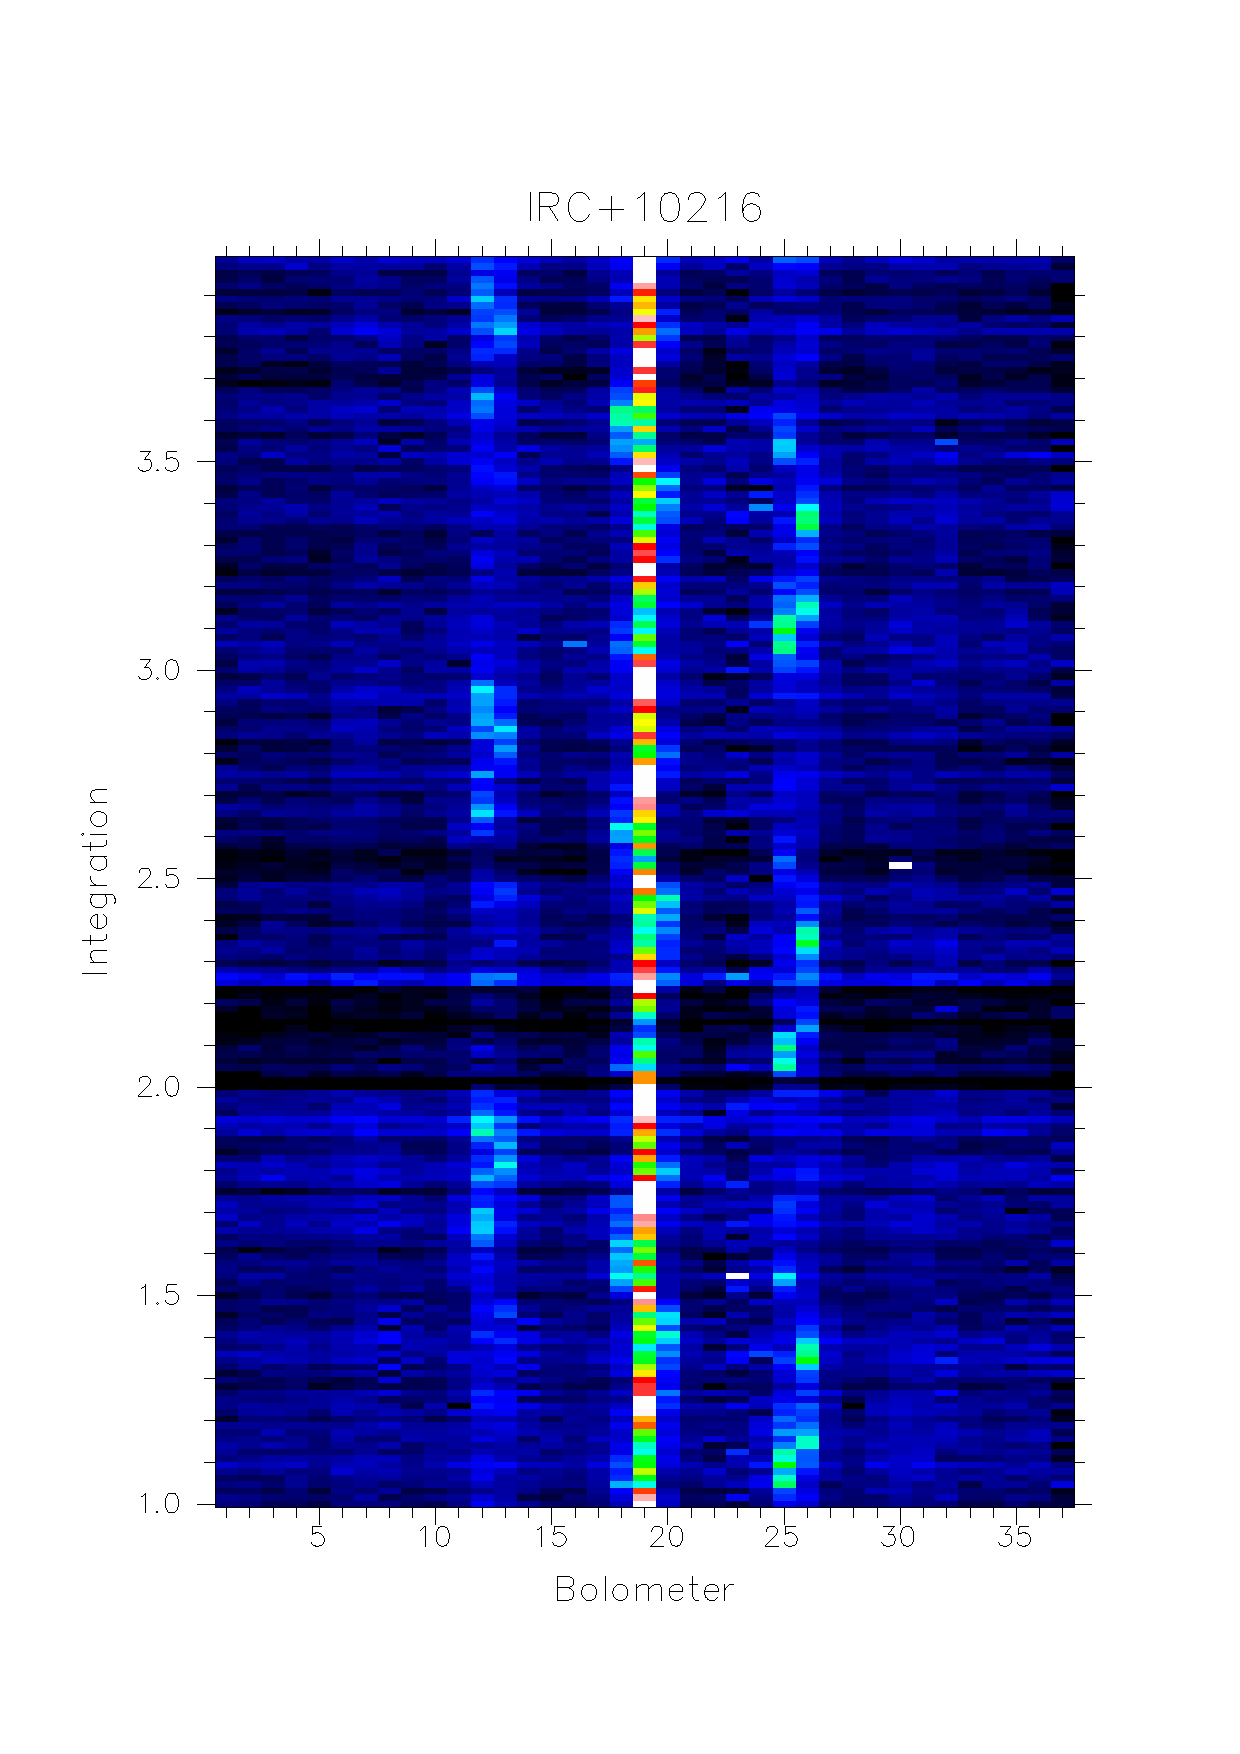
\includegraphics[width=5.4in]{sc11_fig2}
\caption{The extinction corrected data of IRC$+$10216 without
despiking and sky removal.  In this image the bolometers are on the
x-axis and the y-axis is time. A strong signal is seen in the central
bolometer (19) throughout the jiggle cycle, while neighboring
bolometers (12, 13, 18, 20, 25, 26) pick up the signal only during
part of the jiggle cycle. Sky noise variations, which occur at
the same time for all pixels are easily seen, e.g.\ at the beginning
of integration 2.  This image is produced using the \Kappa\ \display\
command with the command line option \it{fill=true}. }

\label{fig:raw}
\end{center}
\end{figure}

From the plot shown in Fig.\ \ref{fig:raw} we can see that the map
suffers from some sky noise, e.g.\ visible as the dark striping at the
beginning of integration 2.  The central bolometer, 19 (h7) shows a
clear signal, and we do not see any really bad (noisy) bolometers,
except perhaps bolometer 23.  Even so, we first need to blank out bad
bolometers.  There are several ways to identify bad bolometers.  The
easiest way, although it may not pick up all noisy bolometers for your
particular map, is to run \scunoise, which is a GUI that allows you to
plot and identify all noisy bolometers using noise measurements done
during the run.  If we do this for the night of 19971208 we find a
total of 9 noise measurements and we can see that some bolometers come
and go, but 23 is always noisy.  From the most nearby noise
measurement, \#88, we find that 23, 32 and 37 have noise levels above
100~nV and 12 is also about twice as noisy as the majority of the
array, which should have a noise level around 40~nV. Before we set
these bolometers to bad we plot the bolometers with \mlinplot\ to
check that these bolometers are indeed noisy in our map.


\begin{myquote}
\begin{verbatim}
% mlinplot i86_lon_ext absaxs=2 lnindx='21:32'
YLIMIT - Vertical display limits /[-0.002588027,0.09385466]/ >
DEVICE - Name of display device /@xwindows/ >
\end{verbatim}
\end{myquote}

In the above example the bolometers 21 -- 32 are plotted as a function
of integration time (Fig.\  \ref{fig:mlin}).  Bolometer 23 is indeed the
noisiest pixel, but 22, and 24 are noisy as well and actually worse
than 32, which was picked up by \scunoise.  Fig.\  \ref{fig:mlin} shows
strong sky noise, which makes it difficult to see the true noise level
of the bolometers, and it is often wise to do a sky noise reduction
(see below), so that one can more easily identify noisy bolometers.
Go through the whole array by choosing suitable bolometer ranges with
the parameter \texttt{lnindx}.  In this example we choose to only
blank out bolometer 23, which we set to bad using \chgqual.
Bolometers 8 and 14 also appear noisy, more so than 12, which we
picked up in the noise measurement, but for the time being we let them
stay.  When we go through the bolometers with \mlinplot\ we can also
see a few spikes, which we will deal with shortly.  Let us now set
bolometer 23 with \chgqual.  Note that we need to surround the file
name with both single and double quotes if we list more than one
bolometer.



\begin{figure}
\begin{center}
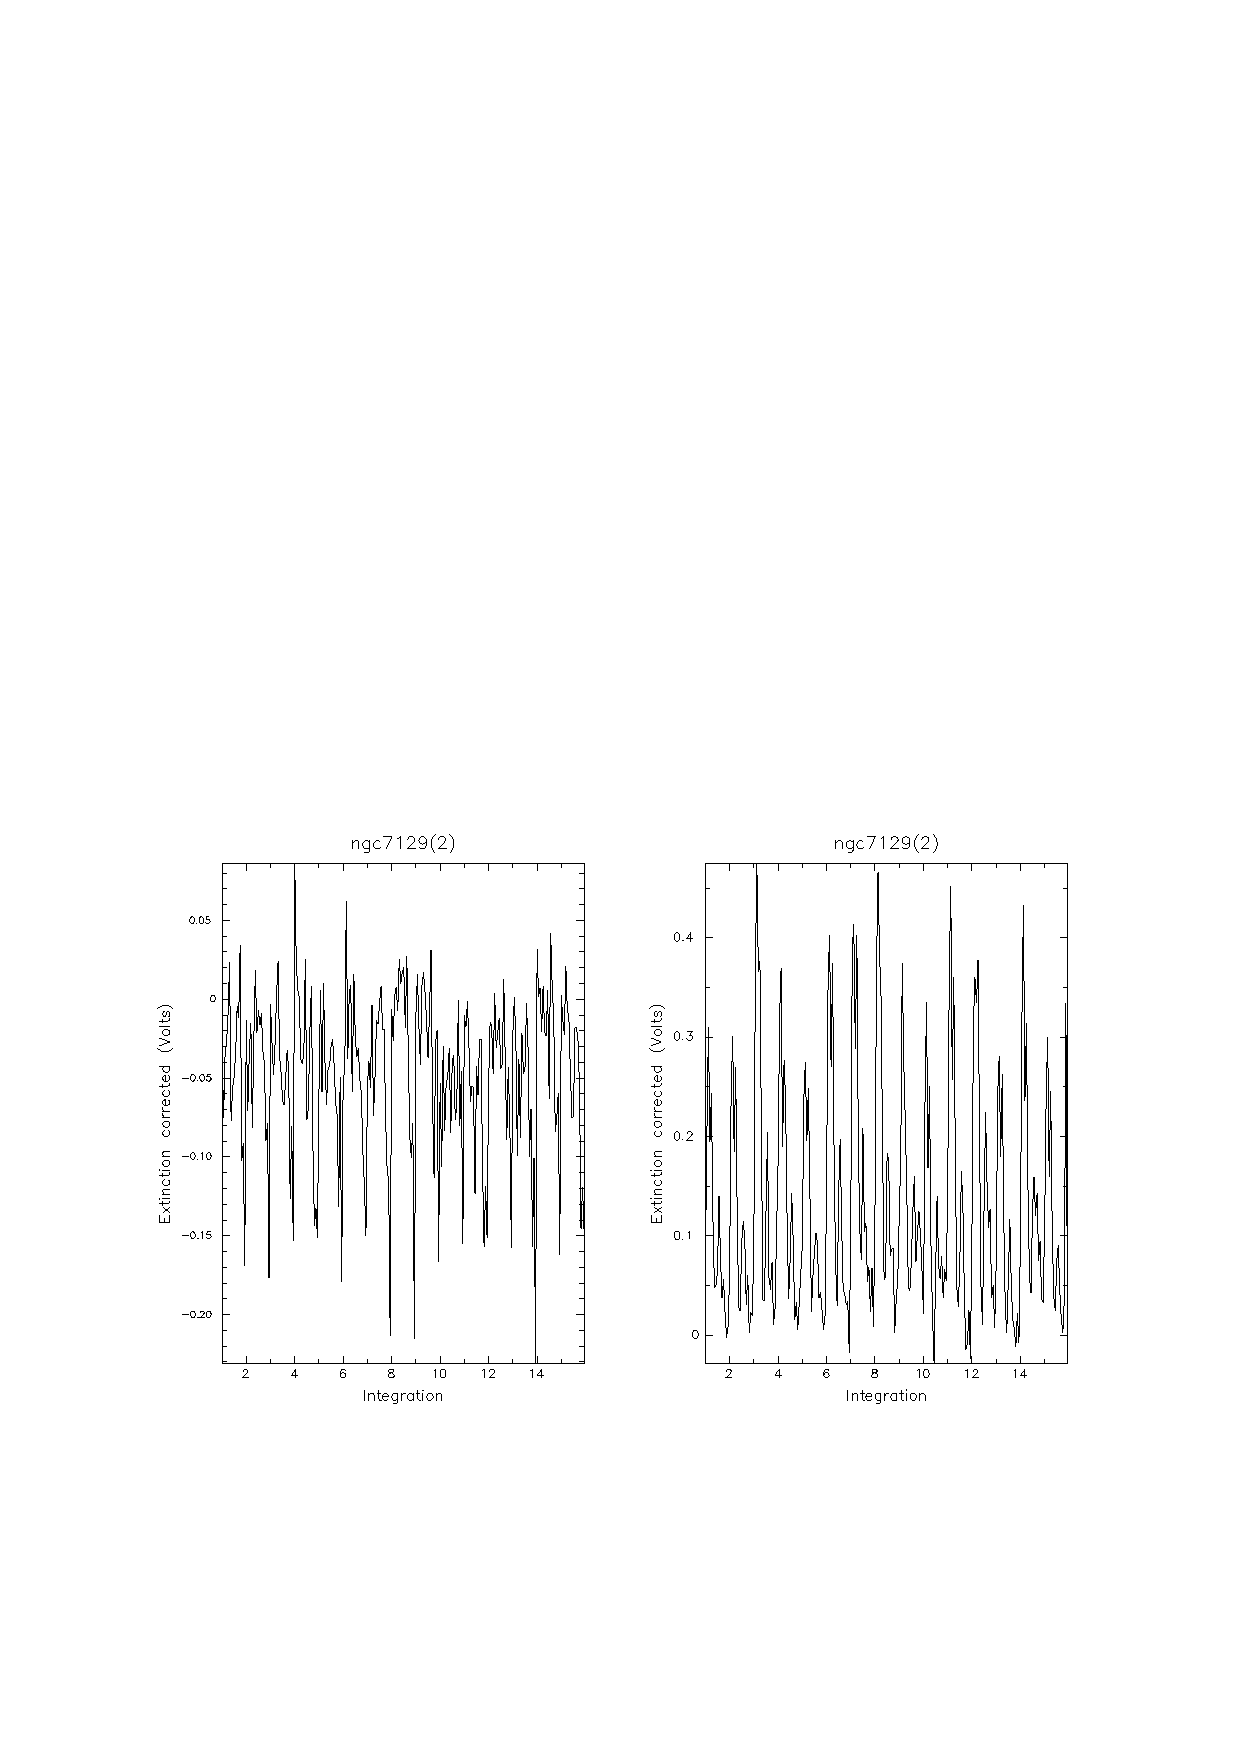
\includegraphics[width=\textwidth]{sc11_fig3}
\caption{Using \mlinplot\ to display a set of bolometers as a function
of time is a good way to identify noisy bolometers.  From this
plot we can see that bolometers 22 -- 24 are noisier than the rest of
the sample.  Note that bolometers 25 and 26, which are in the first
ring surrounding the central bolometer, pick up the source at certain
jiggle positions and this signal should not be confused with noise,
which is random and erratic.  One can also see the strong sky noise
variations, which repeat the same signature for each bolometer, e.g.\
the dip in signal at the beginning of integration 2.}


\label{fig:mlin}
\end{center}
\end{figure}


\begin{myquote}
\begin{verbatim}
% change_quality "'i86_lon_ext{b23}'"
SURF: run 86 was a MAP observation of IRC+10216
SURF: file has data for 37 bolometers, measured at 192 positions.
 - there are data for 4 exposure(s) in 3 integration(s) in 1
measurements.
BAD_QUALITY - Set quality to bad? (No will set quality to good) /YES/
>
\end{verbatim}
\end{myquote}


\subsection{\xlabel{Initial_Sky_Noise_Removal}Initial sky noise
removal \label{Initial_Sky_Noise_Removal}}

As we have already seen, sky noise can be a dominant noise source in a
map, but as long as the sky noise is correlated over the array, it can
be removed.  One can do this in several different ways, but for a
single short integration map one will always use \remsky.  In the
automated SCUBA reduction Jenness et al.\  \cite{Jenness01} use the
median option in \remsky\ and include all bolometers.  Since we have a
centrally symmetric source, we take the second ring, r2, of bolometers
using the median option to avoid spikes that may be present in the
data.


\begin{myquote}
\begin{verbatim}
 % remsky
IN - Name of input file containing demodulated map data
/@o86_lon_ext/ >
SURF: run 86 was a MAP observation with JIGGLE sampling of object
IRC+10216
OUT - Name of output file /'o86_lon_sky'/ >
BOLOMETERS - The Sky bolometers, [a1,a2] for an array
/['4','9','29']/ > r2
SURF: Using 12 sky bolometers
MODE - Sky removal mode /'median'/ >
Sky noise: 0.000602097 (192 points)
Adding mean background level back onto data (value=0.0003676229)
\end{verbatim}
\end{myquote}

Note that the default behavior of this routine is to add the mean bolometer
signal back in to data (this may not be what you wish to do) if it's not then
type:

\begin{myquote}
\begin{verbatim}
% remsky add=false
\end{verbatim}
\end{myquote}


\subsection{\xlabel{InitDespiking}Initial Despiking}

Let us now remove the worst spikes by using the \surf\ task \scuclip\
to take out any spikes exceeding 5 sigma.

\begin{myquote}
\begin{verbatim}
% scuclip
IN - Name of input file containing demodulated map data
/@i86_lon_sky/ >
SURF: run 86 was a MAP observation with JIGGLE sampling of object
IRC+10216
OUT - Name of output file /'i86_lon_clip'/ >
NSIGMA - How many sigma to despike bolometers /5/ >
SURF: Removed 3 spikes
\end{verbatim}
\end{myquote}

\scuclip\ removed 3 spikes in the data, which will do for the moment.



Following despiking and sky removal one can then run \rebin.  The
process of sky removal will significantly improve any maps which have
a `tiled' pattern due to varying sky emission between the two switch
positions.  Below we discuss in more detail how to most efficiently
remove sky noise, which depends on what data sets we have.

\subsection{\xlabel{Sky_Noise_Removal_remsky}Sky noise removal (a)-
\remsky.}

In Section \ref{Initial_Sky_Noise_Removal} we already used \remsky\ to
remove sky noise by choosing a ring of bolometers around the center
and we could even have used all bolometers in the array.  However, for
short chop throws, or where we have an extended source or where the
source is not centered in the array one should be more careful.  A
good way to identify suitable sky bolometers (i.e.\ bolometers without
any source emission) is to convert the map into Az/El (assuming we
chopped in Az) so that we can identify bolometers at the edge of the
array, which are not affected by the chop nor by any source emission.
We regrid the extinction corrected data with the \surf\ task
\rebin, setting the parameter $\rm OUT\_COORDS$ to {\it az}.  In the
example below we use the same data set on IRC$+$10216 as we used
before.  We plot the map immediately with \display\ using the option
{\it faint} and overlay the bolometer array using \scuover\ (use {\it
noname} if you want the bolometers as numbers).


\begin{myquote}
\begin{verbatim}
% display axes clear
IN - NDF to be displayed /@i86_lon_reb/ >
DEVICE - Name of display device /@epsfcol_p/ > xwindows
MODE - Method to define the scaling limits /'fa'/ >
Data will be scaled from -0.0012709096772596 to 0.013754481449723.
% scuover
DEVICE - Name of graphics device /@xwindows/ >
Current picture has name: DATA, comment: KAPPA_DISPLAY.
Using /home/sandell/dec8/i86_lon_reb as the input NDF.
SURF: file contains data for 4 exposure(s) in 3 integration(s) in 1
measurement(s)
\end{verbatim}
\end{myquote}

IRC$+$10216 is extended at 850$\mu$m, because of its large CO
envelope, and we therefore want to use edge pixels away from the chop
direction (usually az) to avoid removing any real signal from the
data.  In our map of IRC+10216 (Fig.\ \ref{fig:irc}) one would
therefore take bolometers 4,9,15 and 22 in the south and 16, 29, and
34 in the north.  If we now run \remsky\ on the extinction corrected
data, we notice that the background level added back to the map was
lower than when we used ring 2, which therefore picks up some of the
faint extended emission surrounding IRC$+$10216.


\begin{myquote}
\begin{verbatim}
 % remsky
IN - Name of input file containing demodulated map data
/@o86_lon_sky/ > o86_lon
_ext
SURF: run 86 was a MAP observation with JIGGLE sampling of object
IRC+10216
OUT - Name of output file /'i86_lon_sky'/ >
BOLOMETERS - The Sky bolometers, [a1,a2] for an array /'r2'/ >
[4,9,15,16,29,34]

SURF: Using 6 sky bolometers
MODE - Sky removal mode /'median'/ >
Sky noise: 0.0005996103 (192 points)
Adding mean background level back onto data (value=6.3598651E-5)
\end{verbatim}
\end{myquote}


\begin{figure}
\begin{center}
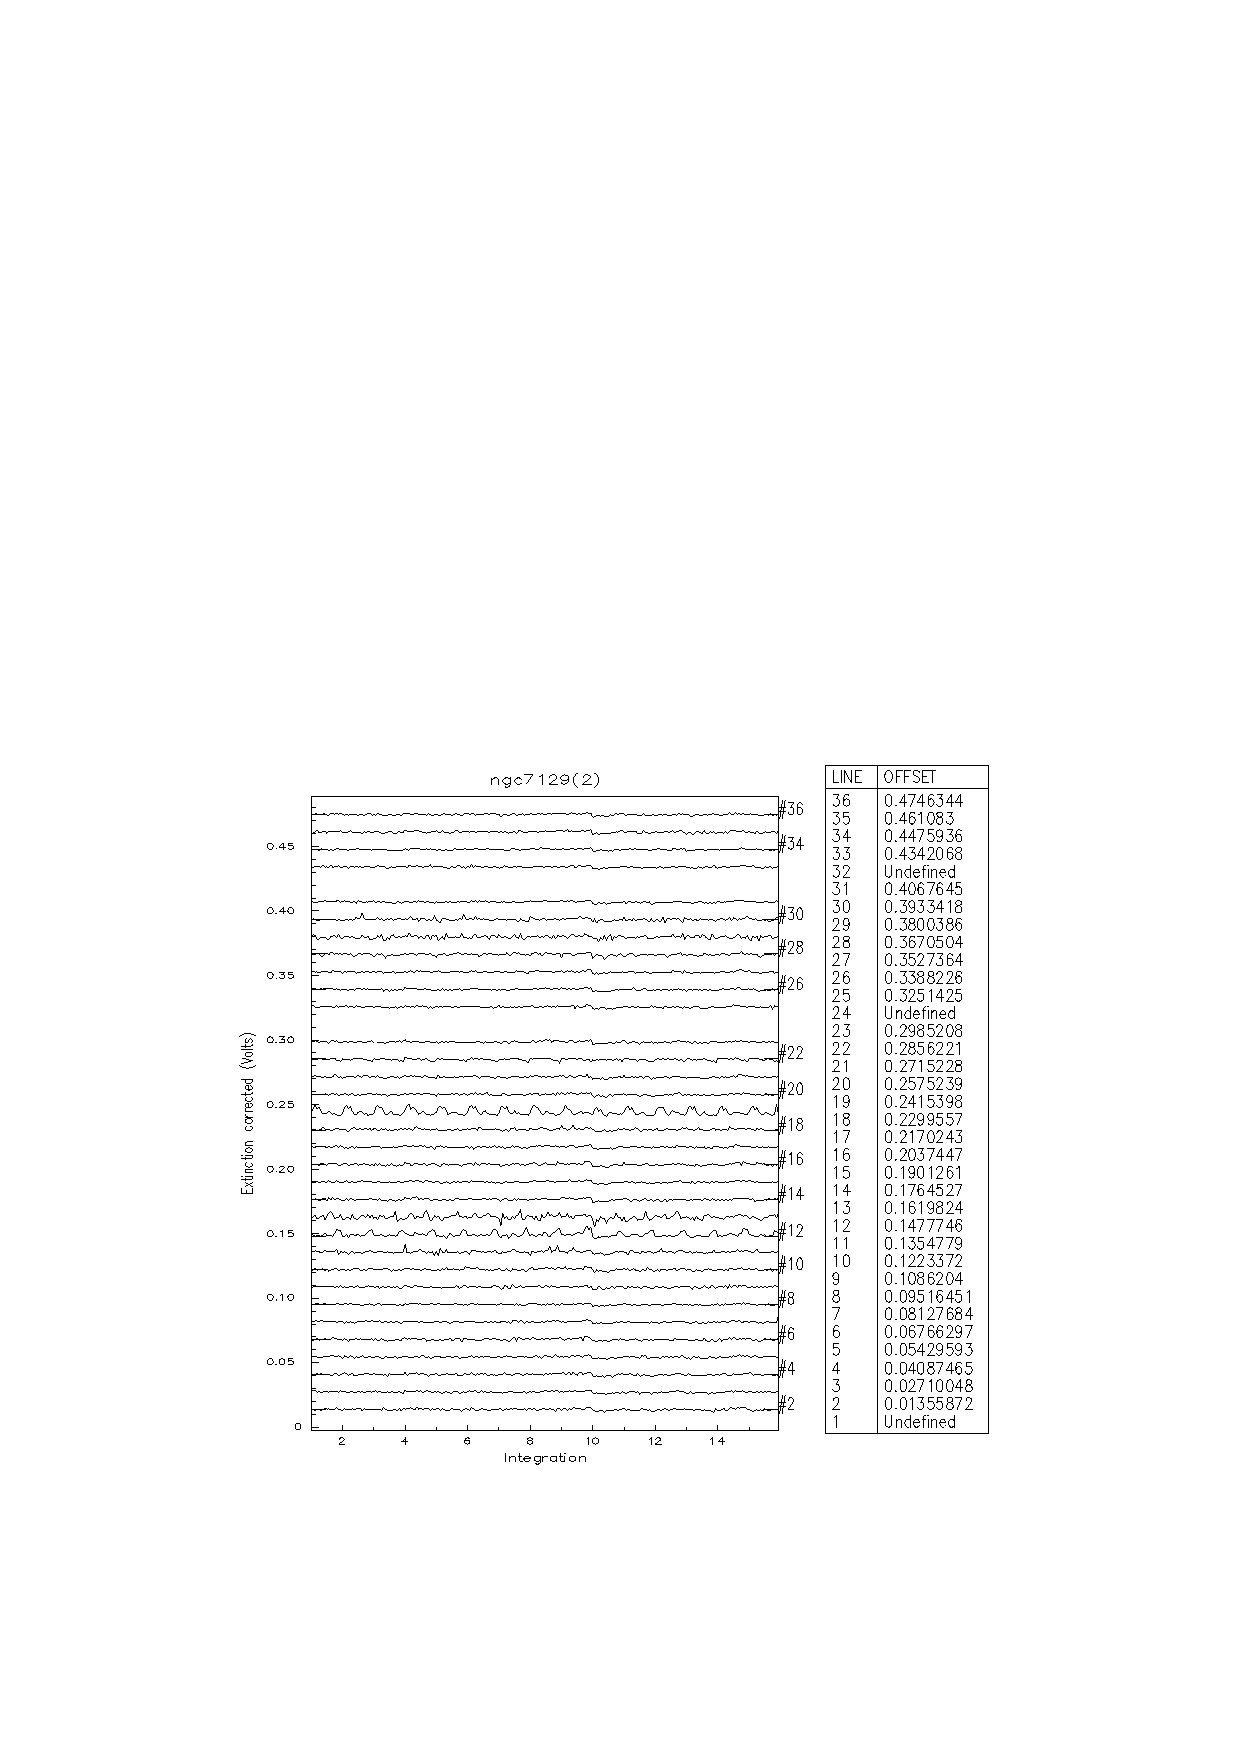
\includegraphics[width=\textwidth]{sc11_fig4}
\caption{This image of IRC+10216 has been regridded in Az/el and
overlaid with the bolometer array in order to allow us to identify
bolometers for sky noise removal. For any extended source we want to
avoid bolometers in the chop direction, and we therefore choose
bolometers at the bottom and top of the map, i.e.\ for example 4,9 and
22 as well as 16, 29, and 34.}
\label{fig:irc}
\end{center}
\end{figure}


\subsection{\xlabel{Sky_Noise_Removal_calcsky}Sky noise removal (b)-
\calcsky \label{Sky_Noise_Removal_calcsky}}

Quite often, especially when we observe galactic sources embedded in
dark or molecular cloud, it is impossible to find any bolometers that
do not pick up source emission.  As long as the source emission is
relatively smooth, this will only affect the mean level in the map,
and any base level that gets removed with \remsky\ can be added back
into the image using $\rm ADD=TRUE$.  But, if there is structure in
the source emission over our sky bolometers, these variations will be
interpreted as sky noise and therefore affect the morphology of our
map.  For extended sources we should therefore use \calcsky.  The task
\calcsky\ computes a model of the source, which it then subtracts from
each bolometer to give an estimate of the sky variation, which is put
into the file extension \texttt{.more.reds.sky}, which can be examined
with e.g.\ \linplot, e.g.,


\begin{myquote}
\begin{verbatim}
% linplot i86_lon_cal.more.reds.sky device=xwindows
\end{verbatim}
\end{myquote}

shows the computed sky noise variations for the scan 86, that we will
re-analyze below (Fig.\ \ref{fig:sky}).


\begin{figure}
\begin{center}
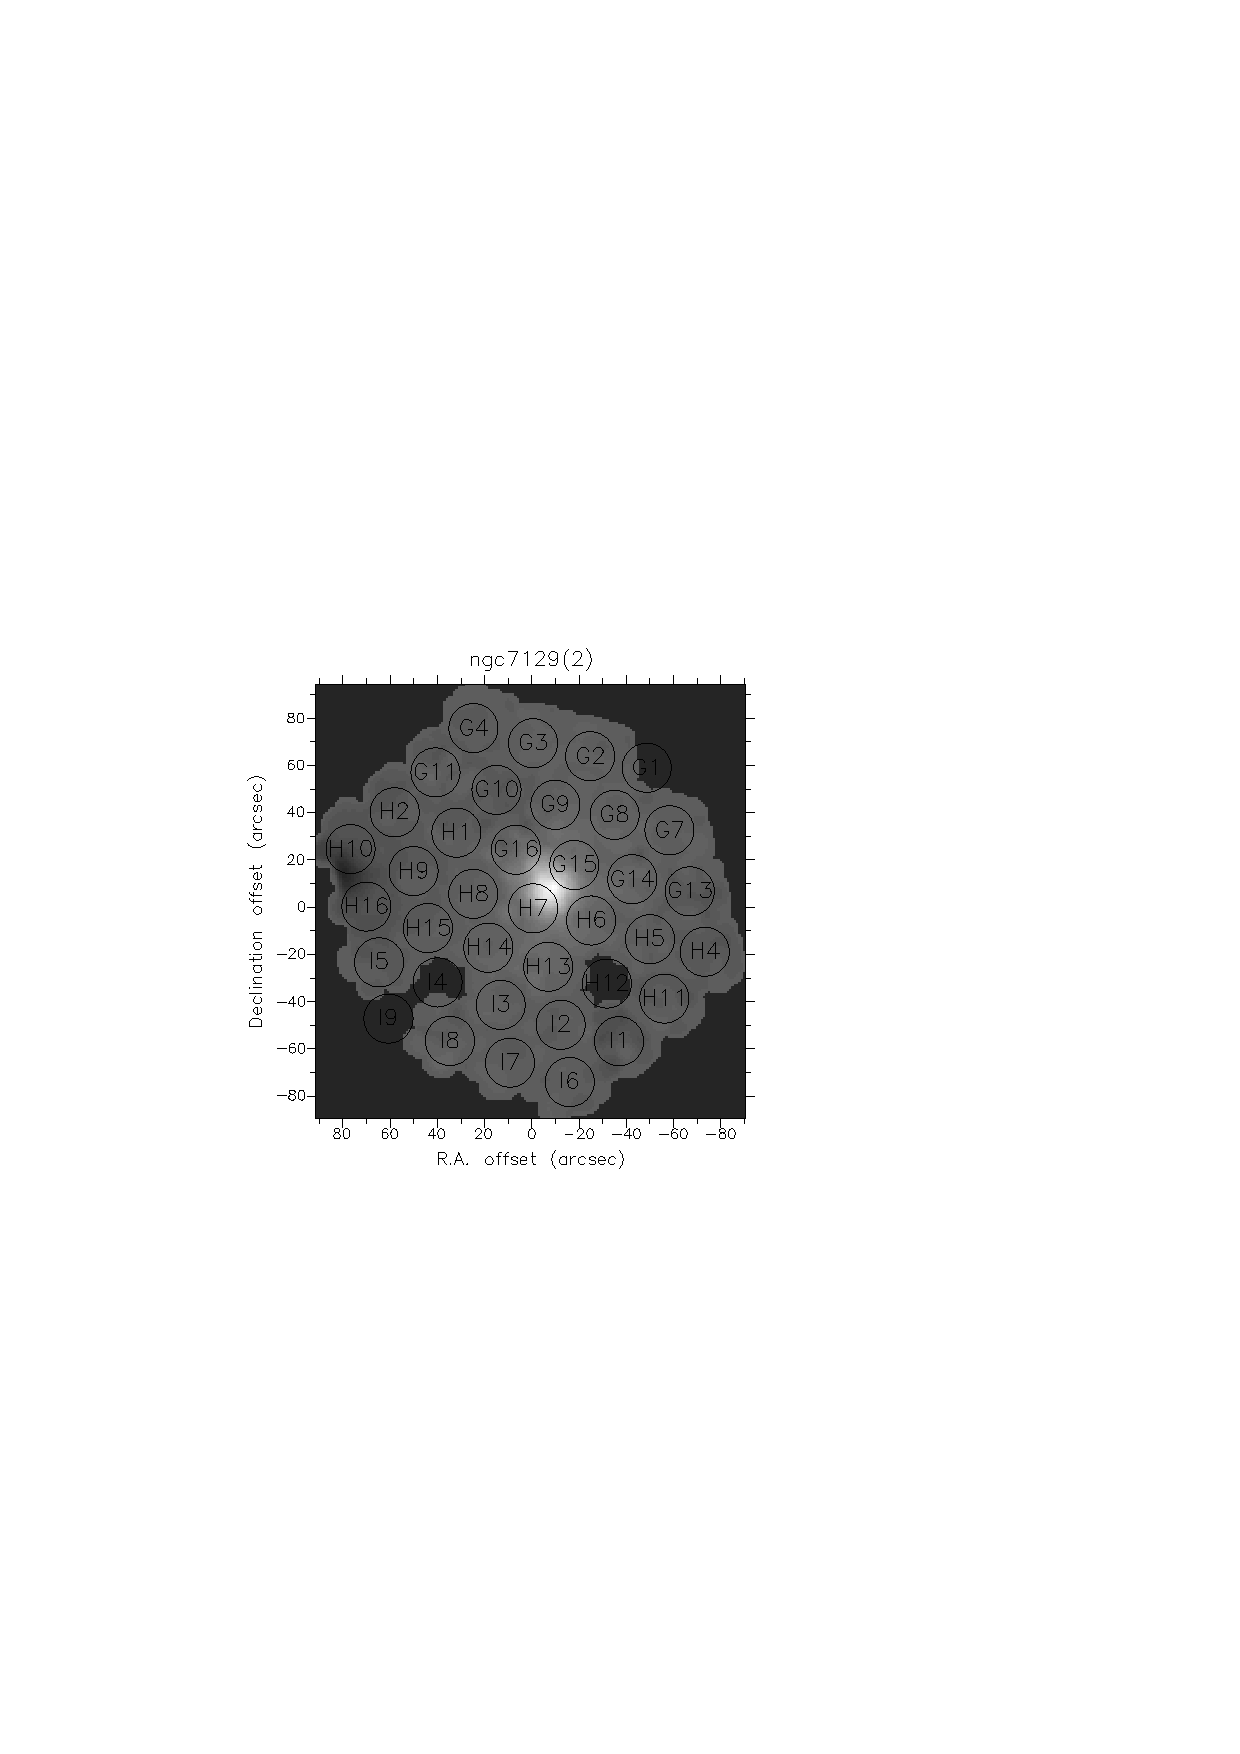
\includegraphics[width=4.0in]{sc11_fig5}
\caption{This plot shows the mean sky variations in scan 86 as computed
by \calcsky\ as a function of time.  Therefore x = 65 corresponds to
start of integration 2 in Fig \ref{fig:mlin}. We can see that it has
clearly picked up the strong sky variations that occur in the beginning
of integration 2 and continued during part of integration 2.  Since
this is a calibrated image, we can see that the sky variations are
extremely strong, and would easily mask a faint source.}


\label{fig:sky}
\end{center}
\end{figure}

We can improve the model by adding data sets to \calcsky\ the same way
as we use \rebin\ for coadding data.  If one has already produced a
final map of the source, one can use this map as the input model for
\calcsky.  For multiple data sets we should make an input file with
weights and offsets as we do for \rebin, see Section \
\ref{Coadding_data}. We now choose the default model, which will be
the median of all the observed maps.  Once \calcsky\ is done, we go
back and run \remsky\ on each data file which was included in the model
computed by \calcsky.

\calcsky\ works extremely well even for extended sources, if one has
kept the chop position fixed. For extended sources it is therefore an
advantage to chop in a fixed ra/dec frame. One can also use \calcsky\
for a spherically symmetric source like IRC$+$10216 even for a chop
throw of 60'', but then one should use {\it az} option for the $\rm
OUT\_COORDS$.  \calcsky\ also includes the option to account for the
chop throw and direction, and it should therefore work even when we
chop differently on extended emission from one map to the next.



For scan maps \calcsky\ is our only option for sky noise removal,
because in scan maps each bolometer will normally include both source
and sky (see later).

Below we show how to use \calcsky\ on the same file we already reduced
with \remsky. When we now run \remsky\ it will not ask for sky
bolometers, but will use the sky extension stored in the header to
remove sky noise variations.


\begin{myquote}
\begin{verbatim}
% calcsky
OUT_COORDS - Coordinate sys for sky determination /'RJ'/ >
SURF: output coordinates are FK5 J2000.0
REF - Name of first data file to be processed /'i86_lon_sky'/ >
i86_lon_cal
SURF: run 86 was a MAP observation of IRC+10216 with JIGGLE sampling
SURF: file contains data for 4 exposure(s) in 3 integrations(s) in 1
measurement(s)

WEIGHT - Weight to be assigned to input dataset /1/ >
SHIFT_DX - X shift to be applied to input dataset on output map
(arcsec) /0/ >
SHIFT_DY - Y shift to be applied to input dataset on output map
(arcsec) /0/ >
IN - Name of next input file to be processed /!/ >
SURF Input data: (name, weight, dx, dy)
   -- 1: i86_lon_cal (1, 0, 0)

BOXSZ - Size of smoothing box (seconds) /2/ >
MODEL - File containing source model /!/ >
% remsky
IN - Name of input file containing demodulated map data
/@i86_lon_ext/ >
SURF: run 86 was a MAP observation with JIGGLE sampling of object
IRC+10216
OUT - Name of output file /'i86_lon_sky'/ > i86_lon_sky
REMSKY: Using SKY extension to determine sky contribution
\end{verbatim}
\end{myquote}

The sky noise we see in our jiggle maps is due to changes in the sky
emission between nods of the telescope.  For unstable sky conditions
this results in a tile-pattern in your map.  This type of structure
will not be removed by \calcsky\ if we apply it to a single data set.
Indeed in this particular example, \remsky\ with selected sky
bolometers gave a much better result than using \calcsky.  However,
for really extended sources and scan maps we may not have a choice.
We will have to use \calcsky\ followed by \remsky.

Another advantage of \calcsky\ which is worth mentioning is that we
can run \calcsky\ on the 450$\mu$m array and copy the calculated sky
noise variations to the 850$\mu$m array after appropriate scaling.
This enables us to remove sky noise variations on a very faint
extended 850$\mu$m--source, without subtracting out source emission.

\subsection{\xlabel{Despiking} Manual Despiking}

The way we despike jiggle maps depends on whether we have done short
or long integrations and on whether our source is compact or extended.
In the above example we only have 3 integrations and \desp\ will miss
most spikes.  We can still use \scuclip\, but if we want to go deep,
we have to make sure that we don't clip the source as well.  We know
that IRC$+$10216 is relatively compact with a faint `halo' type
emission surrounding the core.  It may therefore enough to use
\scuclip, but go deeper than in our initial despike effort.  To be on
the safe side, i.e.\ to make sure that we do not clip the source, we
set the central bolometer to bad before we start and reset it back to
good afterwards using \chgqual.


\begin{myquote}
\begin{verbatim}
% change_quality 'i86_lon_sky{b19}'
SURF: run 86 was a MAP observation of IRC+10216
SURF: file has data for 37 bolometers, measured at 192 positions.
 - there are data for 4 exposure(s) in 3 integration(s) in 1
measurements.
BAD_QUALITY - Set quality to bad? (No will set quality to good) /YES/
>
% scuclip
IN - Name of input file containing demodulated map data
/@i86_sho_sky/ >
SURF: run 86 was a MAP observation with JIGGLE sampling of object
IRC+10216
OUT - Name of output file /'i86_lon_clip'/ >
NSIGMA - How many sigma to despike bolometers /5/ > 4
SURF: Removed 10 spikes
% change_quality 'i86_lon_clip{b19}'
SURF: run 86 was a MAP observation of IRC+10216
SURF: file has data for 37 bolometers, measured at 192 positions.
 - there are data for 4 exposure(s) in 3 integration(s) in 1
measurements.
BAD_QUALITY - Set quality to bad? (No will set quality to good) /YES/
> no
\end{verbatim}
\end{myquote}

Compared to our first 5 sigma we now found 10 additional spikes.  We
could probably have used 3 sigma, but with a small data set it is
better to be conservative, For the short array, we have to be really
careful when using \scuclip, if we work with 64--point jiggle maps.
If we are looking at a point source centered in the array, the jiggle
steps are so large, that the first ring of bolometers will pick up the
source in part of the jiggle pattern.  \scuclip\ can in this case
interpret the source as being noise, since it only shows up in a just
a couple of points, and flag them.  The end result can easily be that
when we regrid the map, we get an artificially narrow image, because
we despiked the ``flanks'' of the source.  If we want to run \scuclip\
on the short array, we should not only blank the central bolometer,
but also the first bolometer ring (seven bolometers), and then reset
the flagged bolometers afterwards and despike them manually, which
becomes somewhat tedious.


For short maps on strong or extended objects we therefore mostly end
up doing manual despiking.  We can either use the interactive shell
script \dspbol\ or the \Figaro\ routine \sclean.

\begin{myquote}
\begin{verbatim}
% sclean
IMAGE - (IMage) Name of image to be cleaned /o86_lon_sky/ >
o86_lon_sky
OUTPUT - (OUTput) Name of resulting image /o86_lon_clip/ >
o86_lon_clip
IDEV - Device for image display /'xwindows'/ >
\end{verbatim}
\end{myquote}

which will give you an image similar to Fig.\  \ref{fig:clean}.
\sclean\ is an interactive application and if you select the xwindow,
and type `b' while the cursor is over a selected bolometer you will
get the display shown in Fig.\  \ \ref{fig:clean}.  Here the left hand
side shows all the bolometers, and the right hand side shows just the
bolometer you selected.  The two most useful commands are probably `a'
- delete the pixel selected, and `y' - delete the indicated area and
fix by interpolation along the y-axis.  Manual despiking like this is
usually only needed for short integration maps of strong sources or
when taking out more extended glitches in scan maps, which are not
picked up by automatic despiking.


\begin{figure}
\begin{center}
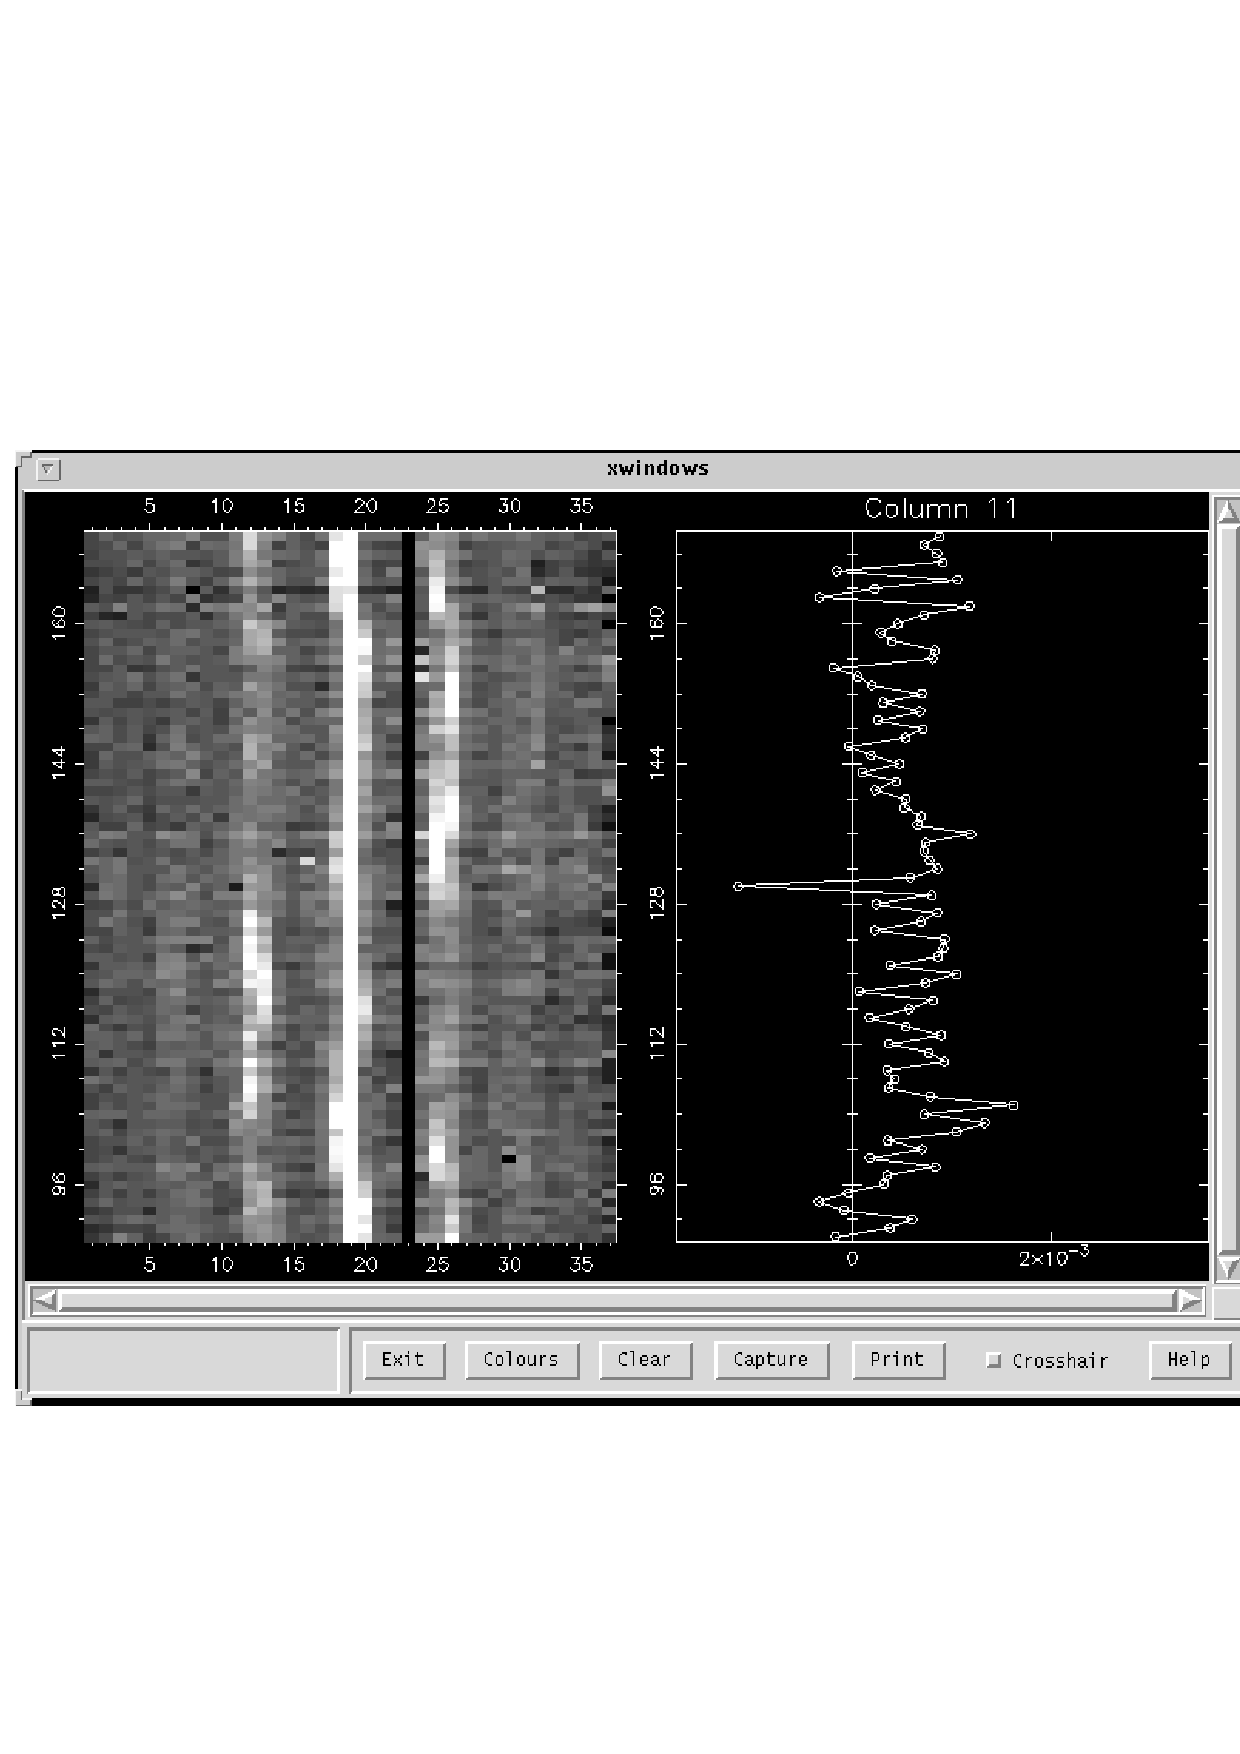
\includegraphics[width=6in]{sc11_fig6}
\caption{The display from the \Figaro\ package \sclean. \sclean\ allows
you to easily inspect the time series data and despike data. }
\label{fig:clean}
\end{center}
\end{figure}



\subsection{\xlabel{Pointing}Pointing corrections and final map
creation}

Before we create our final \rebin, we will still need to calibrate the
map (Section \ \ref{Calibration}) and correct for pointing drifts that
occurred over the map. Since we have only dealt with a single map so
far, we omit the calibration stage and proceed to correct for pointing
drifts. To do this we reduce the closest pointing observations before
and after the map in the same way as we reduced our map, but with
minimal despiking and regridding the pointing map in {\it az}.  These
pointing errors we find have to be negated in the task \chgpnt. For
scan 86 I find one pointing done on the star itself before the map
(\#81), and none afterwards. The final pointing errors of \# 81 are
DAZ/DEL = 0.38''/+0.33'' at an LST of 9:26 as deduced from the FITS
header of that scan. These errors are the residual from on-line
pointing corrections and off-line data reduction of scan 81. If we
treat our map as if it was a pointing observation we find pointing
errors of +1.52''/+0.12'', which we apply directly after negating the
sign as shown below. Instead of choosing a time halfway through the
map, we have to take the LST time at the end of the map.  This is kind
of cheating, because we derive pointing from the same objects that we
are supposed to correct the pointing for, but here we do it only to
illustrate how pointing corrections are done.

\begin{myquote}
\begin{verbatim}
% change_pointing
IN - Name of input file containing demodulated map data
/@i86_lon_sky/ > i86_lon_clip
SURF: run 86 was a MAP observation of IRC+10216
SURF: observation started at LST 9 41 05 and ended at 9 50 09
SURF: no pointing corrections found

CHANGE_POINT - Do you want to change the pointing correction data > y
POINT_LST - The sidereal time of the pointing offset (hh mm ss.ss)
/!/ > 9 26
POINT_DAZ - The azimuth pointing correction to be added (arcsec) >
-0.38
POINT_DEL - The elevation pointing correction to be added (arcsec) >
-0.33
POINT_LST - The sidereal time of the pointing offset (hh mm ss.ss)
/!/ > 9 50 10
POINT_DAZ - The azimuth pointing correction to be added (arcsec) >
-1.52
POINT_DEL - The elevation pointing correction to be added (arcsec) >
-0.12
POINT_LST - The sidereal time of the pointing offset (hh mm ss.ss)
/!/ >
\end{verbatim}
\end{myquote}

We can now run the sky noise corrected, despiked, and pointing corrected data
through \rebin\ to obtain our final map \textit{i86\_lon\_reb}.  Looking at
the map, we can see that bolometers, which we knew  were noisy still can
be seen, but since we do not have any additional data sets to add to the map,
we will leave the map as such.  The pointing offsets, as determined with
\centroid\ give pointing offsets of -0.18'' in RA and 0.0'' in Dec, suggesting
that the pointing corrections worked quite well.

Now we would do the short array in the same way either by re--running
\scuquick\ or by starting with the \surf\ task \ext. We now run \ext\
on \texttt{i86\_flat}, which was created when we reduced the long
array, and which also contains the flat fielded data for the short
array.

\subsection{\xlabel{Coadding_data}Coadding data, or how to deal with
long integrations \label{Coadding_data}}

Reducing multiple observations of the same source is about as easy as
reducing a single map, it is just a bit more time consuming. Some
aspects of the reduction process, like despiking, now becomes simpler
and more reliable.

All the basic steps up to and including sky removal are done the same
way as in the example above, but now we can despike differently,
because we have much more redundant data.  After we have extinction
corrected, calibrated, done sky removal and pointing corrections we
can now try \desp\ on all the data sets.


To demonstrate \desp\ we have collected 10 jiggle maps with two or
three integrations of HL~Tau, one of our secondary calibrators.  All
the maps are taken in good weather conditions, but some suffer from
sharp variations in sky noise. We have set the really noisy bolometers
to bad for all maps, but in some cases we have still left bolometers
with 1.5 - 2 times the average noise level.  For all maps the chop
throw was 120" in Azimuth.  Note that if you chop on the array this
despiking technique will not work very well, unless you use a fixed
chop angle, or regrid in {\it az} which works very well for a point
source or a centrally condensed spherically symmetric source. To make
the reduction easier, and to enable us to go back and redo the
despiking, we make a small ASCII file for the maps, which includes the
name, weight and pointing shift -- one line per map.  Here we start
without applying pointing corrections because the pointing errors are
negligible.  Neither do we apply weighting, because we will need
despiked maps in order to compute the weights.  In this example we
call the file \texttt{hl.inp}.  The first line in this file is
\texttt{hl39\_lon\_sky 1 0 0}, where {\it hl39\_lon\_sky} is the file
name and 1 is the weight.  The two zeros that follow the weight are
the pointing shifts in the coordinate frame that the data are rebinned
to, which in this case {\it RJ}. Since HL~Tau is a point source with
negligible extended emission one could equally well have rebinned the
whole data set in {\it az}. We are now ready to try \desp.

\begin{myquote}
\begin{verbatim}
% despike noloop
OUT_COORDS - Coordinate sys of output map; PL,AZ,NA,RB,RJ,RD or GA
/'RJ'/ >
SURF: output coordinates are FK5 J2000.0
REF - Name of first data file to be rebinned /'hltau_lon'/ > hl.inp
SURF: Reading file hl39_lon_sky
SURF: run 39 was a MAP observation of HLTau with JIGGLE sampling
SURF: file contains data for 4 exposure(s) in 3 integrations(s) in 1
measurement(s)

   ...............   list continues until it has read in all maps,
then

SURF Input data: (name, weight, dx, dy)
   -- 1: hl39_lon_sky (1, 0, 0)

     ..............
   -- 10: hl42_lon_sky (1, 0, 0)

NSIGMA - Sigma levels at which to despike /3/ >
SMODE - Smoothing mode for clipping envelope (none,hann) /'hann'/ >
DEVICE - Name of graphics device /@xwindows/ >
DMODE - Display mode (Spiral, Xlinear, Ylinear, Diag1, Diag2)
/'spiral'/ >
XRANGE - X range of plot (! to continue) /[1,5112]/ > 1,2000
XRANGE - X range of plot (! to continue) /[1,2000]/ > !
SURF: 8 spikes detected in file hl39_lon_sky
...........................
SURF: 196 spikes detected in file hl42_lon_sky
OUT - Name of despiked data file /'hl39_lon_dsp'/ >
...........................
OUT - Name of despiked data file /'hl42_lon_dsp'/ >
\end{verbatim}
\end{myquote}



\begin{figure}
\begin{center}
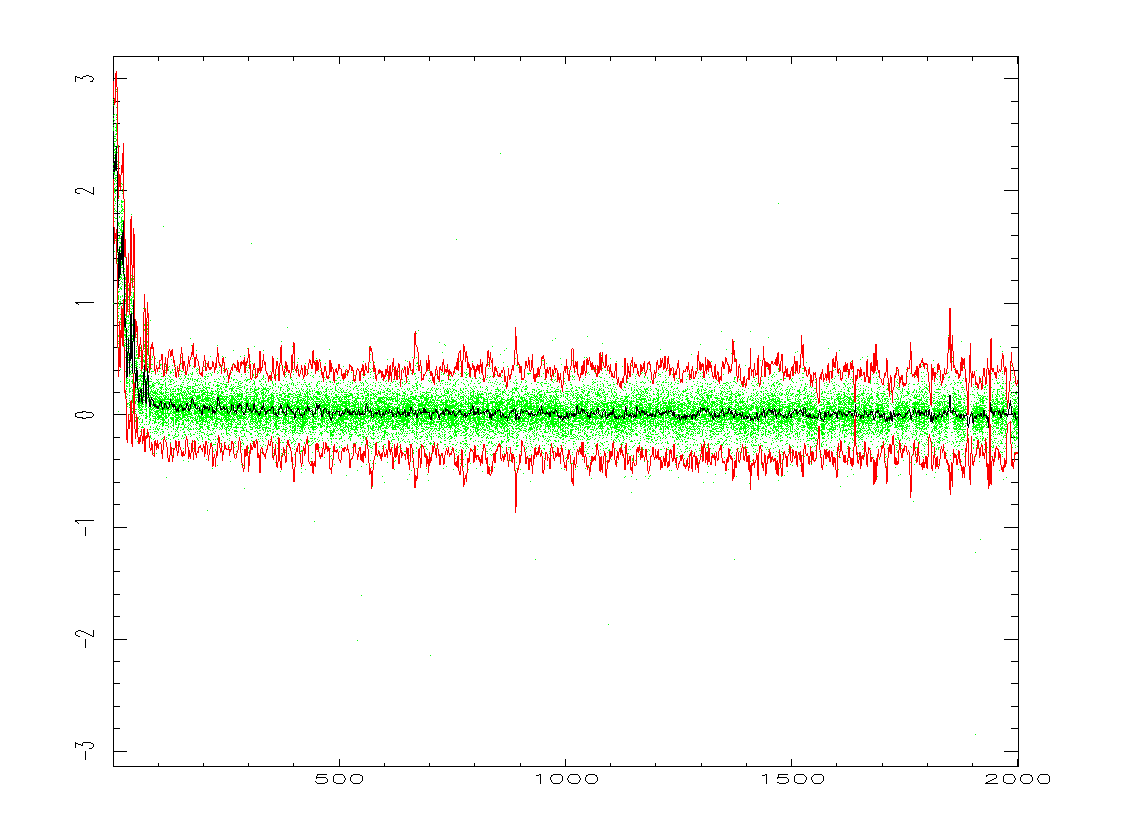
\includegraphics[width=4in]{sc11_fig7}
\caption{These are the first 2000 data points analyzed by \desp. The
observed data are plotted in green, median in black and the Hanning
smoothed 3--$\sigma$ envelope is plotted in red. Any data points
outside this limit will be flagged as bad.}
\label{fig:desp}
\end{center}
\end{figure}


The display for the first 2000 data points are shown in Fig.\ \ref{fig:desp}.
Note that after you run \desp\ the display may get messed up.  It is normally
sufficient to clear the display with \gdclear\ and re-issue the the color
table, e.g.\ \lutbgyrw.  If there are still problems, delete the \agi-file
from your home directory (\texttt{agi\_xxx.sdf}, where \texttt{xxx} is the
name of your work station).


We now run \rebin\ on each data set to determine the offsets we need to center
the map, which will ensure that we get the sharpest possible image.  We also
determine the rms noise level for each map.  Here it is a clear advantage to
use \gaia.  After displaying the map with your preferred color scheme and
contrast level using the \texttt{View} menu, go to the \texttt{Image-Analysis}
menu and click on \textit{image regions}.  Choose the polygon option of
\textit{ARD regions} and outline the region you want to use with the cursor.
After it is done, click on \textit{Stats selected} and you are done.  For
determining pointing offsets it is easier to use the \Kappa\ command
\centroid\ i.e.\ \texttt{centroid search=19 cerror}, where we adjust the
search parameter to minimize the fit errors.  For 850~$\mu$m and a 1~arcsec
cell setting \textit{search} to 17 or 19 generally gives a good result.  After
we have determined the noise level and position offsets for each map we
compute the weights for each map.  An easy way to do this is to set the weight
for the first map equal to one.  All other maps are then weighted relative to
this map.  If we call the integration times t$_1$ and t$_2$, and the
corresponding noise values n$_1$ and n$_2$ for map 1 and map 2 respectively,
then we can compute the weighting factor from the following equation:

\begin{equation} weight = (n_1/n_2)^2\times(t_1/t_2) \end{equation}

\noindent
We now edit in the weights and position offset in \texttt{hl.inp} and
run \desp\ again on the original data set.  The end result appears
good enough.

Now we can form the final co-add of the data very easily, since we
have already computed the weights and position shifts that we need to
get the best S/N and sharpest image from our data.  The only thing we
need to do is to change the file extensions from {\it sky} to {\it
dsp}, the name we used for despiked data files.  We rename the input
file to \texttt{hl.dsp} in case we would like to redo the despiking.
We now run this file through \rebin, i.e.,


\begin{myquote}
\begin{verbatim}
% rebin noloop
REBIN_METHOD - Rebinning method to be used /'LINEAR'/ >
SURF: Initializing LINEAR weighting functions
OUT_COORDS - Coordinate sys of output map; PL,AZ,NA,RB,RJ,RD or GA
/'RJ'/ >
SURF: output coordinates are FK5 J2000.0
REF - Name of first data file to be rebinned /'hl42_lon_dsp'/ >
hl.inp
SURF: Reading file hl39_lon_dsp
SURF: run 39 was a MAP observation of HLTau with JIGGLE sampling
SURF: file contains data for 4 exposure(s) in 3 integrations(s) in 1
measurement(s)
..................
SURF: Reading file hl42_lon_dsp
SURF: run 42 was a MAP observation of HLTau with JIGGLE sampling
SURF: file contains data for 4 exposure(s) in 3 integrations(s) in 1
measurement(s)

SURF Input data: (name, weight, dx, dy)
   -- 1: hl39_lon_dsp (1, 0.08, 1.19)
   -- 2: hl64_lon_dsp (0.4, 0.64, 0.75)
   -- 3: hl41_lon_dsp (0.9, -0.23, 2.7)
   -- 4: hl55_lon_dsp (1, -0.86, 0.38)
   -- 5: hl61_lon_dsp (0.8, 0.14, 1.04)
   -- 6: hl75_lon_dsp (0.75, 0.4, -0.13)
   -- 7: hl84_lon_dsp (0.5, 0.42, 0.83)
   -- 8: hl60_lon_dsp (0.9, 0.11, -1.41)
   -- 9: hl23_lon_dsp (0.75, 0.1, 0.46)
   -- 10: hl42_lon_dsp (0.3, 0.75, 1.06)

LONG_OUT - Longitude of of output map centre in hh (or dd) mm ss.ss
format
/'+04 31 38.46'/ >
LAT_OUT - Latitude of output map centre in dd mm ss.ss format
/'+ 18 13 57.8'/ >
OUT_OBJECT - Object name for output map /'HLTau'/ >
PIXSIZE_OUT - Size of pixels in output map (arcsec) /3/ > 1
SIZE - Number of pixels in output map (NX,NY) /[194,192]/ >
OUT - Name of file to contain rebinned map /'HLTau'/ > hltau_lon
WTFN_REGRID: Beginning regrid process
WTFN_REGRID: Entering second rebin phase (T = 3.113513 seconds)
WTFN_REGRID: Entering third rebin phase (T = 14.55025 seconds)
WTFN_REGRID: Regrid complete. Elapsed time = 15.23921 seconds
\end{verbatim}
\end{myquote}

We now have our final co-added map, which is almost as good as it
can get from the data we had available.

If you have extremely large data sets, then you may find that your
computer runs out of memory in \rebin.  The recommended solution, if
you cannot find a more powerful workstation, is to split the data set
in two parts, run each separately through \rebin, and co-add the two
final maps using the \Kappa\ command \add\ or the task \makemos\ in
\ccdpack.


\section{\xlabel{Scanmaps}Scan maps}

Scan maps, i.e.\ mapping while continuously scanning the array over the
source, require a few additional steps in the reduction procedure. The
reduction process is also different depending on whether we made
conventional scan maps or used the ``Emerson2'' technique.
Conventional scan maps refer to maps done while chopping in the scan
direction and restoring the resulting dual beam map with the
EKH algorithm (the Emerson-Klein-Haslam algorithm -- known to all who
have ever used \nod\ or \jcmtdr\ \cite{jcmtdr}) before transforming the
map into equatorial coordinates.  The ``Emerson2'' technique is
essentially a basket weaving technique, where one can scan in an
arbitrary angle but chop in two orthogonal directions and restore the
dual beam map in the Fourier plane after converting the dual beam maps
to equatorial coordinates. This method therefore requires a minimum of
two maps, one where we chop in RA and one where we chop in Dec. The
standard setup for SCUBA is to use six maps, three of which are done
while chopping in RA with chop throws of 30, 44 and 68'', and three
while chopping in Dec with the same three chop throws. The chop throws
are chosen so that we should be sensitive to most spatial frequencies
in the map. If possible one should try to choose the map size so that
it covers the whole source and provides an additional baseline region
off source, but as we all know this is not always possible.

For all scan maps we can do the first three reduction steps: \resw,
\flatf, and \ext, the same way as we would do for any jiggle map.  We
also blank out noisy bolometers, but from here onwards we need to
apply slightly different methods.  Scan maps are also affected by sky
noise, especially when we use the ``Emerson2'' technique.  This is
because the time difference between when the positive and the negative
beam passes the same position on the sky can be significant, and
sometimes even longer than in jiggle-maps.  This is especially
noticeable for large maps and large chop throws.  We can crudely
remove sky noise in scan maps, but not as well as in jiggle maps,
\calcsky\ is our main tool and needs several repeats of the same maps
to work efficiently.


\subsection{\xlabel{despiking_scan_maps}Despiking}

After we have extinction corrected the map and taken out noisy
bolometers, we need to despike the data.  This is done with the \surf\
task \desp2, which takes a small portion from each end of a scan and
computes the rms--variations for each bolometer and then does a
standard sigma clip.  If you want to be conservative, use 4 sigma.
This does a reasonable job, but large spikes (extending over several
seconds in time) are not detected and these will have to be removed
manually using \sclean\ or \dspbol.  It is often necessary to run
\desp2 a second time after \scanrlb, because even with the same sigma
threshold, the rms is now smaller and one finds a fair amount of
residual spikes missed in the first round.


\subsection{\xlabel{Base_line_removal}Base line removal - \scanrlb}

The SCUBA on-line software normalizes each scan in conventional (EKH)
scan maps, which leads to baseline offsets, but even the ``Emerson 2''
maps have baseline uncertainties.  Spillover, large spikes and sky
noise add to these baseline uncertainties.  It is therefore absolutely
necessary to remove the baseline offset for each bolometer.  If it is
omitted one may end up with severe striping in the map.  If your map
is large enough, i.e.\ you have no source emission at the end of your
scan, you can run \scanrlb, and fit a linear baseline for each scan
(exposure and bolometer) by taking the end portions of the scan as a
measure of the signal level.  The default size of the region used for
the baseline subtraction is the number of data points in one chop
throw.  This can be inadequate for the small chops, especially if the
data are spiky or suffer from sky noise variations, and you may
consider increasing the default to perhaps 100''.  The output from
\scanrlb\ is the basic map name, now appended by \texttt{\_rlb}, which
is the file you will use as an input for the next stage in the data
reduction.


However, if your map is not large enough to start and end on a region
free of emission \scanrlb\ will result in a gradient over the scan.
Taking the default behavior of \scanrlb\ in this situation
is probably the leading cause of poor results obtained from scan
mapping.  When you map galactic regions it is usually better to use
the median rather than the default, which is \textit{linear}.  Another,
sometimes more successful approach is to use \scuba\ sections.

In scan map mode each `sweep' or `raster' is a section (exposure), and
the complete map is an integration. If you believe that you have
sections of the map that are free of emission, you may be in luck, and
you can use these emission free sections to provide the baseline level
for the rest of your map. To find out which section is which, display
your rebinned map and then use \scuover. To produce the image in Fig.\
\ref{fig:moon} we typed:

\begin{myquote}
\begin{verbatim}
%display 20000721_0023_lon_reb
DEVICE - Name of display device /@xwindow/ >
MODE - Method to define the scaling limits /'SCALE'/ >
LOW - Low value for display /-0.86096328496933/ >
HIGH - High value for display /12.873136520386/ >
% scuover exposure=1
DEVICE - Name of graphics device /@xwindow/ >
Alignment has occurred within the AXIS Domain.

NDF - Image to display bolometers over /@20000721_0023_lon_reb/ >
SURF: file contains data for 21 exposure(s) in 1 integration(s) in 1
measurement(s)
\end{verbatim}
\end{myquote}

One can see that the scan map started at the top right of the map (a
scan map of the moon's limb) and took 11 `sweeps' or exposures to
complete the map.  One can see that only exposures 1, 9, 10 and 11
started and ended off source.  Therefore when one wishes to remove the
baselines (remembering that one now has to go back 2 or 3 steps to do
this) from this image the best method would be:

\begin{myquote}
\begin{verbatim}
% scan_rlb
IN - Name of input file containing demodulated data
/@20000721_0023_lon_ext/ >
SURF: run 23 was a MAP observation of object MOON
SURF: file contains data for 21 exposure(s) in 1 integration(s) in 1
measurement(s)
OUT - Name of file to contain restored data /'20000721_0023_lon_rlb'/
>
METHOD - Method to use for baseline removal /'LINEAR'/ > section
RLB - Remove fitted baseline from output data /YES/ >
SECTION - Please enter a section (including {}) > [{e1}{e9}{e10}{e11}]
REMOVE_DC_OFFSET_SECTION: Processing integration 1
\end{verbatim}
\end{myquote}

Its obvious with a source like the moon when you are on and off source
and because the moon fills most of the image, the data were
additionally masked.  This is a rather special case, where it would
have been very difficult to do the baseline subtraction any other way
without ending up writing special purpose software.  For molecular
clouds and star forming regions it is often very difficult to find
emission free regions.  For really extended emission, like the
Galactic center, it was therefore found that the best way to do
baseline removal is to use the median level of all the scans for each
bolometer (Pierce-Price et al.\  \cite{Pierce00}), which corresponds to
specifying SECTION as \{\}.  Quite often you will find that you have to
do an initial map reduction to see how extended the region is and
where you can find emission free areas.  Once you know this, it is
much easier to go back to noisy sub-maps and redo the baselines.


\begin{figure}
\begin{center}
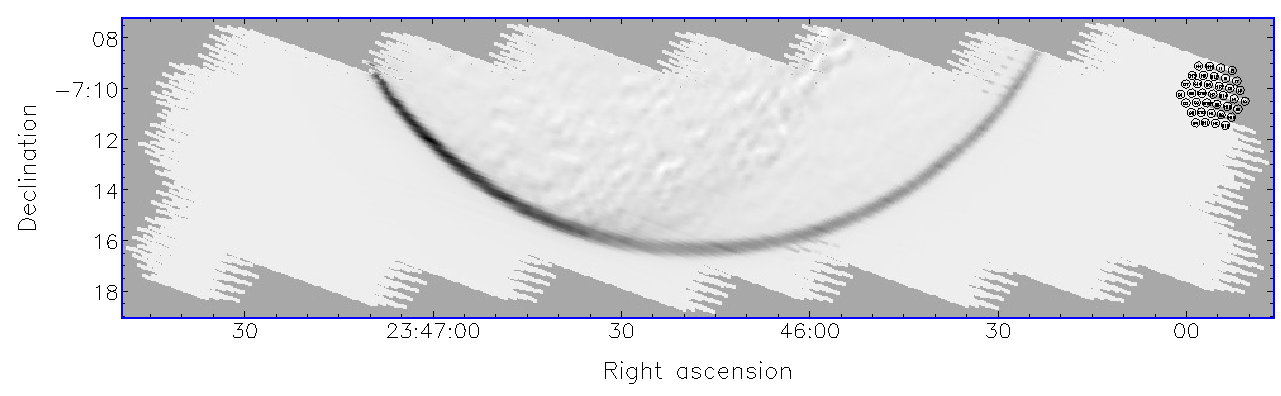
\includegraphics[angle=-90,width=\textwidth]{sc11_fig8}
\caption{An example of a scanmap of the moon's limb. The SCUBA
array's position at the beginning of the observation is shown.  In
total it took 11 `sweeps' or exposures to map the area requested.}

\label{fig:moon}
\end{center}
\end{figure}

\subsection{\xlabel{scan_maps_calcsky}Sky noise removal in scan maps
\label{scan_maps_calcsky}}

There are no sky bolometers in a scan map, i.e.\ each bolometer can be
on source, and furthermore a bolometer will cover a different region
of the sky for each map exposure.  It is therefore not possible to
remove sky noise the way we usually do for jiggle maps.  Sky noise can
be extremely severe and rapid on Mauna Kea.  Under such circumstances
sky noise variations can completely distort a scan map, especially for
large chop throws.  \calcsky\ was originally developed to give us a
technique for reducing sky noise in scan maps, but as we have seen it
works also quite well for jiggle maps, as discussed in Section
\ref{Sky_Noise_Removal_calcsky}.  \calcsky\ computes a model of the
source emission, and subtracts it from the data for all bolometers as
a function of time. Several maps can be co-added.


Below we test \calcsky\ on a small scan map, taken with a 20'' chop
in RA.  The map file, {\it rn14\_lon\_dsp} has already been baseline
subtracted, pointing corrected, calibrated and despiked.


\begin{myquote}
\begin{verbatim}
% calcsky
OUT_COORDS - Coordinate sys for sky determination /'RJ'/ >
SURF: output coordinates are FK5 J2000.0
REF - Name of first data file to be processed
/'rn14_lon_reb'/ > rn14_lon_rlb
SURF: run 14 was a MAP observation of RNO1b with RASTER sampling
SURF: file contains
SCULIB_PROCESS_BOLS: no data for exp 7 in int 1, meas 1
SCULIB_PROCESS_BOLS: no data for exp 7 in int 2, meas 1
SCULIB_PROCESS_BOLS: no data for exp 7 in int 3, meas 1
WEIGHT - Weight to be assigned to input dataset /1/ >
SHIFT_DX - X shift to be applied to input dataset on output map
(arcsec) /0/ >
SHIFT_DY - Y shift to be applied to input dataset on output map
(arcsec) /0/ >
IN - Name of next input file to be processed /!/ >
SURF Input data: (name, weight, dx, dy)
   -- 1: rn14_lon_rlb (1, 0, 0)

BOXSZ - Size of smoothing box (seconds) /2/ >
MODEL - File containing source model /!/ >
\end{verbatim}
\end{myquote}

We can now examine the sky variations with \linplot. There seems to be
clear systematic variations as a function of time, but the maximum
deviation is only $\sim$ 150 mJy/beam, c.f. the jiggle map we did
earlier (Fig.\ \ref{fig:sky}), which showed sky noise variations of
about 600 mJy/beam.

However, we can easily check how much we gain in noise performance if
we remove the sky noise from the data.  We therefore run \remsky\ on
the same data file that we processed with \calcsky.

\begin{myquote}
\begin{verbatim}
% remsky
IN - Name of input file containing demodulated map data
/@rn14_lon_reb(280:340,90:300)/ > rn14_lon_rlb
SURF: run 14 was a MAP observation with RASTER sampling of object
RNO1b
OUT - Name of output file /'rn14_lon_sky'/ >
REMSKY: Using SKY extension to determine sky contribution
\end{verbatim}
\end{myquote}

In this case the gain was rather marginal. The despiked data file gave
an rms noise of 70 mJy/beam after running it through \rebin\, while the
sky corrected one improved by $\sim$ 0.5 mJy/beam (i.e.\ an improvement
of less than one percent), when examined over the same area of the map,
which means that it was not really worth doing. Nevertheless, I go
through all six maps in the set, and find as I had expected the largest
sky fluctuations for maps taken with a 65'' chop throw. In the last map
of the set (65'' chop in Dec), the maximum sky fluctuations were $\sim$
250 mJy/beam, or  peak--to--peak sky noise variations of $\sim$ 500
mJy/beam, resulting in a 7\% improvement in noise after subtracting the
calculated sky noise variations.

\calcsky\ does not work very well on a single map, but since \calcsky\
can account for the chop throw, one can use a first version of the
final map as a model for the individual sub--maps.  If necessary, one
can do a second iteration by using the sky corrected sub--maps to
create a new improved map, which can be used as an even better model
for \calcsky.

{\it From here onwards the rest of the reduction differs depending on
the scan map mode.}

\subsection{\xlabel{Conventional_scan_maps}Conventional scan maps}

After we calibrated the maps and done the baseline removal, we need to
restore the map from a dual to a single beam map.  This is done by
using \restore.  This task does a standard EKH restoration.  Below we
show an example of restoring a scan map of NGC\,7538, a high mass star
forming region.  In this case we accept the default for the chop
throw, but if the restored map looks poor, it is most likely because
the chop throw deviates from the nominal value.

\begin{myquote}
\begin{verbatim}
% restore
IN - Name of input file containing demodulated data /@n39_lon_rlb/ >
SURF: run 39 was a MAP observation of object NGC7538
CHOP - Size of chop /60/ >
SURF: file contains data for 8 exposure(s) in 2 integration(s) in 1
measurement(s)
OUT - Name of file to contain restored data /'n39_lon_res'/ >
2POS_DECONV: Processing exposure 1 of integration 1
...........
SCULIB_2POS_DECONV : no data for exp 8 in int 1, meas 1
2POS_DECONV: Processing exposure 1 of integration 2
 ..........
2POS_DECONV: Processing exposure 7 of integration 2
SCULIB_2POS_DECONV : no data for exp 8 in int 2, meas 1
\end{verbatim}
\end{myquote}

Once this is done, we can apply pointing corrections to remove any
pointing drifts we had during the duration of the map.  If the map is
still uncalibrated (we strongly recommend to apply calibration
immediately after the extinction correction), we should do it now.
Once we have all the maps calibrated we can proceed and co-add any
additional maps that we may have using \rebin, exactly like we do for
jiggle maps.  Note that if you co-add data sets taken in different
weather conditions or during different nights, you will have to weight
the individual data sets in order to minimize the noise in your final
map.


\subsection{\xlabel{Emerson2_maps}Scan maps taken with the
``Emerson2''
technique}

Scan maps taken with the ``Emerson2'' technique, i.e.\ basket weaving
in Fourier space, have to be run through \rebin\ without restoring
them from dual to single beam maps and in the same coordinate system
that was used for the chop throw (e.g.\ RJ or PL).  You have to make
one map for each chop throw and each map has to have identical
dimensions and pixel size.  We recommend that you make the maps larger
than the area mapped and then cut them in size after running them
through \remdbm, the final reduction stage for ``Emerson2'' scan maps.
Since \remdbm\ makes use of fast Fourier transforms, it is advisable
to choose map sizes, which are a power of two.  Make sure that you do
not choose a size equal to the default size for any of the sub--maps,
because in that case \rebin\ will choose its own map center, which is
not equal to the center pixel of the map. The end result will be a
garbled map.  To make it easy to identify the map sets we need for
\remdbm\ one can give the calibrated, noise weighted and co-added maps
names like : {\it m30ra.sdf, m44ra.sdf, m30dec.sdf, m44dec.sdf etc.},
not because the tasks need it, but it easier for book keeping
purposes.  These maps also have to be corrected for pointing drifts
but they should not be restored.  The maps are still dual beam maps
and each source in the map should show up as a positive and a negative
feature in the image.  Fig.\ \ref{fig:dual} shows the first sub--map
of RNO1b, i.e.\ scan {\it rn14\_lon\_sky}, which we used to test
\calcsky\ in Section \ref{scan_maps_calcsky}.  It has now run through
\rebin\ and given a size 384 $\times$ 384 with a pixel size of 1''.
Since this map was taken with a 20'' chop in RA, we called it {\it
ra20.sdf}.  We should have made the map slightly bigger, because the
maps with 30'' and 65'' chops will cover a larger area.  Note that
this map was taken at a time when the recommended chop throws were
20'', 30'', and 65'', now the recommended minimum set is 30'', 44''
and 68'', which gives a somewhat better recovery of spatial
frequencies.



\begin{figure}
\begin{center}
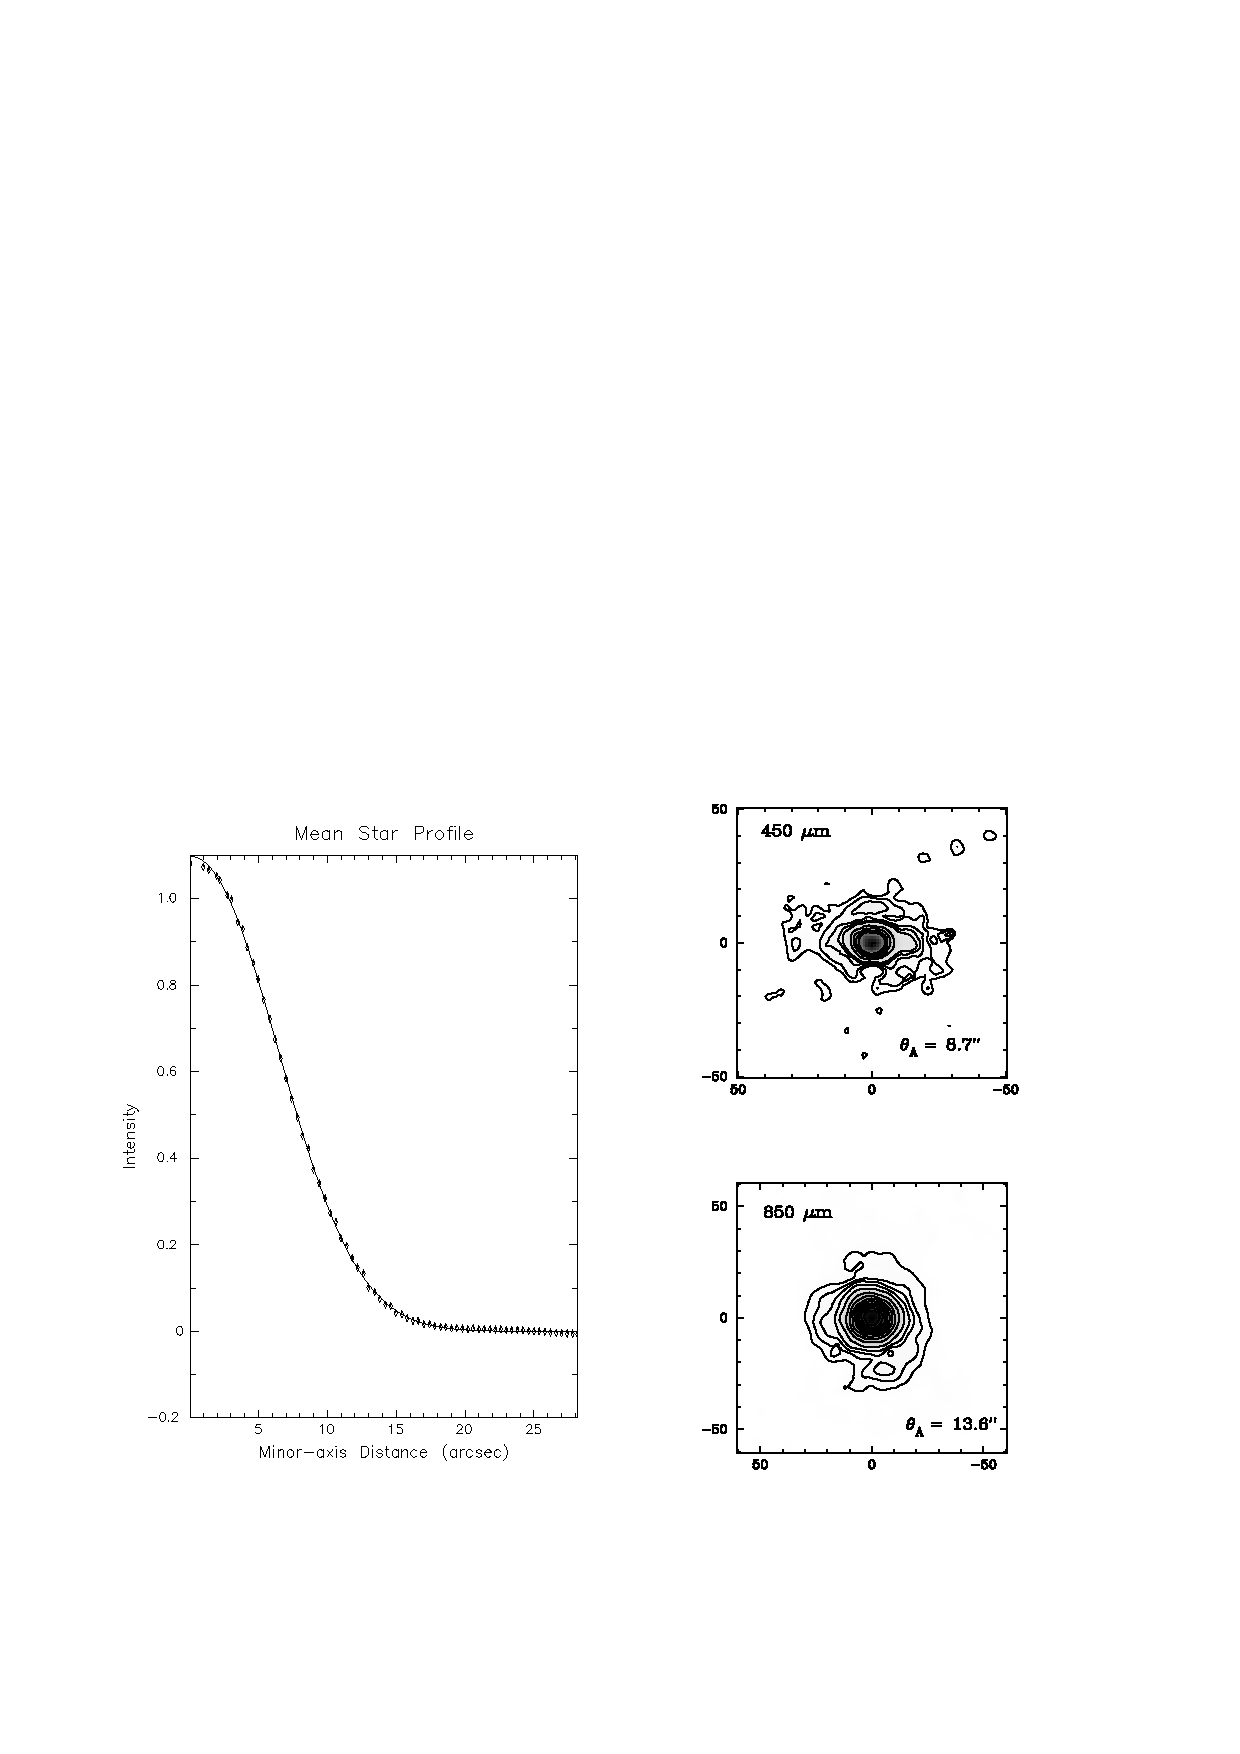
\includegraphics[width=\textwidth]{sc11_fig9}
\caption{An example of the first map in a series of 6 maps taken
with the ``Emerson2'' mapping technique. This is a calibrated map
with a 20" chop in RA, which is converted to RJ with \rebin\, but
still unrestored. We can see the positive and the negative features
in the map, and a few noise spikes at the edges of the map. }
\label{fig:dual}
\end{center}
\end{figure}


Once we have all maps pointing corrected and co-added to the same
pixel size and dimension, we can run \remdbm\, which converts the maps
into our final image.  In the example below I take the six sub--maps
of RNO1b and convert them into a map called {\it rno1b\_lon\_reb}
using \remdbm.  We specify the name of the final map with the parameter
\texttt{out}, and a provide the task with a listing of the files, see
below:


\begin{myquote}
\begin{verbatim}
% remdbm ra20 ra30 ra65 dec20 dec30 dec65 -out=rno1b_lon_reb
Perl/ADAM messaging is present. Good
Starting monoliths...Done
Loop number 1
Chop: PA=90 THROW=20

Doing forward transformation
....................................................

Loop number 6
Chop: PA=0 THROW=65

Doing forward transformation

There was 1 element changed in the Data array.
Running inverse FFT...
Maximum difference between estimates of the same Fourier component is
0.02118739.

Doing inverse transformation

Result stored in rno1b_lon_reb
ADAM exited

\end{verbatim}
\end{myquote}

\remdbm\ also accepts wild--cards and we could therefore have listed
the files as {\it ra* dec*} and it would have picked up the whole set
of six maps.  Neither do we have to give it chop throw or chop
direction.  It will extract that information from the FITS--header.
The task can restore a single map file, but even two maps in
orthogonal directions looks rather ugly, and it is strongly
recommended to use a set of 4 or 6 maps.


Due to the way the Fourier transformations are done, \remdbm\ forces
the sum of all pixels to be zero.  This will introduce a small
negative background level in the map.  We can remove this baseline by
analyzing the map with \Kappa's \stats\ or with \gaia\ and add back
the level we deduce with \cadd.  For our map we find the negative
baseline to be $\sim$ 0.3 Jy/beam, which we add to the map.  The
final, baseline subtracted map is shown in Fig.\ \ref{fig:final}.




\begin{figure}
\begin{center}
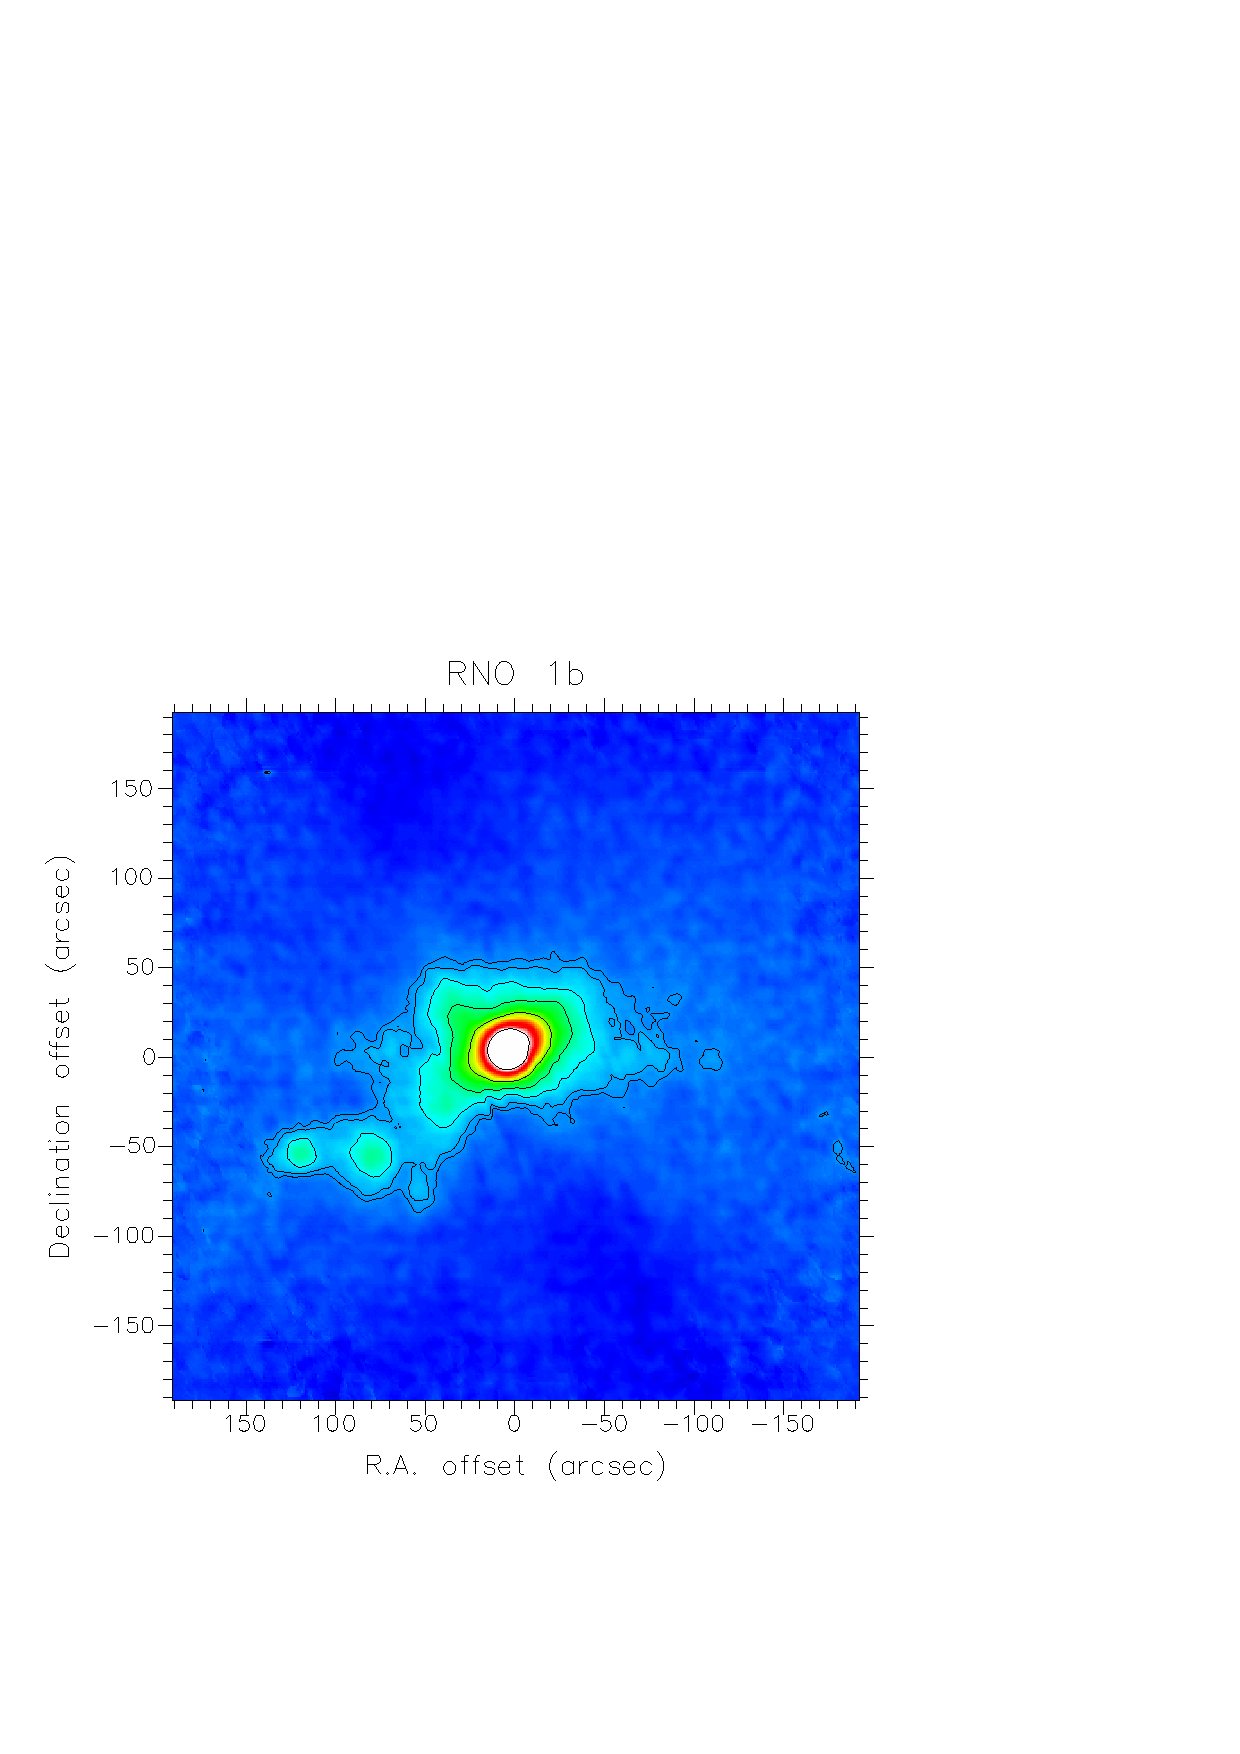
\includegraphics[width=\textwidth]{sc11_fig10}
\caption{Our final ``Emerson2'' scan maps of RNO 1b. The map has a
little bit of negative residuals in the scans that went over the
strongest part of the map (edge of the map at p.a. $\sim$ 30 and 210
degrees), indicating that the baseline removal was not perfect, but it
does not show up with the contrast used for this figure. For a
published version of the map, see Sandell and Weintraub \cite{Sandell01}.}
\label{fig:final}
\end{center}
\end{figure}

\section{\xlabel{Calibration} Map calibration  \label{Calibration}}


\begin{figure}
\begin{center}
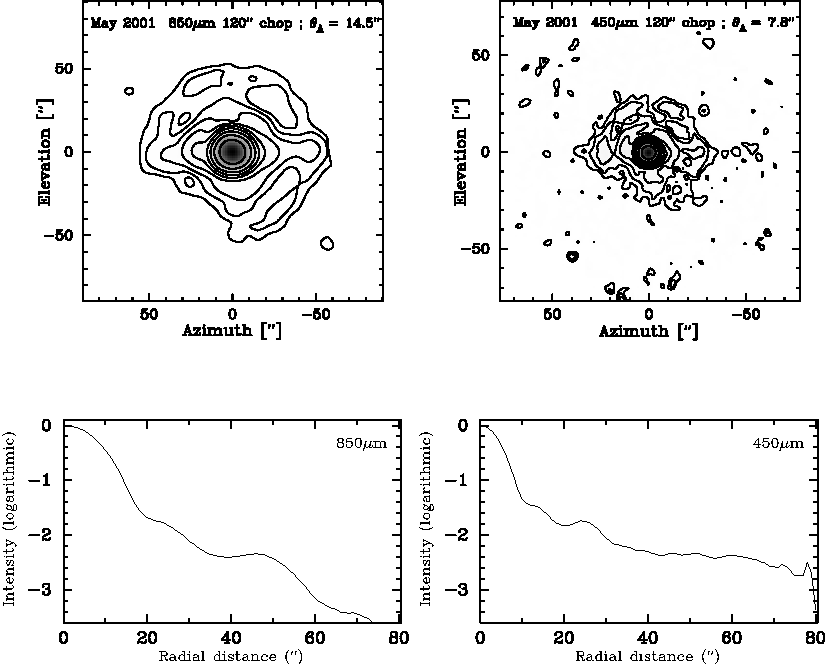
\includegraphics[width=\textwidth]{sc11_fig11}
\caption{Upper panel: Logarithmic contour plots of Uranus beam maps
overlaid on grayscale.  At 850 $\mu$m we plot ten contours starting
from 0.25\% of the peak intensity, while the 450 $\mu$m beam map goes
from 1\% of the peak intensity.  One can see a diffraction like ring
in the 850 $\mu$m map at a radius of $\sim$ 47'', but the amplitude is
$<$ 1\% of the peak.  At 450 $\mu$m the ring is at $\sim$ 25'' and has
an average amplitude of $\sim$ 2\% of the peak intensity.  This is
seen more clearly in the lower panels, which show radially averaged
beam profiles plotted in a logarithmic scale}

\label{fig:beams}
\end{center}
\end{figure}



Until now we have deliberately avoided the issue of calibrating your
data. This means that your reduced data, up until this stage, are in
units of volts. Since the calibration varies from night to night and
even within a single night, one should generally calibrate individual
maps before coadding to achieve the best result. So how does one
convert instrumental units into a physical measure of luminosity or
surface brightness? The solution as in most astronomy is to look at a
source of known brightness in exactly the same way, i.e.\ using the
same mode of observing for your target as well as for your
calibrator(s).

In the optical and infra-red the standard sources are almost always
point sources, standard stars, and the point spread function is well
defined.  In the submillimetre things are more complicated.  Our
primary calibrators, Mars and Uranus, are not point sources, and the
point spread function is very extended and strongly wavelength
dependent.  The JCMT beam at 450 $\mu$m is actually much worse than
the ill-fabled Hubble before the mirror was corrected.

The way we calibrate may differ depending on whether we observe point
sources or extended sources.  For point sources we can ignore the
error beam and do simple aperture photometry, for extended sources we
normally have to calibrate in Jy/beam and characterize our beam
profile.  In the following we first go through how to characterize the
beam profile, then the case of calibrating in Jy/aperture and finally
we proceed to the more general case of calibrating in Jy/beam, which
is valid for all cases.


\subsection{\xlabel{beam_profiles} Analyzing beam maps
\label{beam_profiles}}

The calibration differs for jiggle maps and scan maps and it is also,
although more weakly, dependent on chop throw.  The relatively large
difference in calibration for scan maps is due to the different chop
wave form used for scan maps.  The difference between a jiggle map
with a 120'' chop throw compared to one with a 60'' chop throw is
mostly dictated by duty cycle and to a lesser extent by changes in the
beam.  The beam is slightly broader with a 120'' chop throw, but the
duty cycle (time spent on source) is also slightly lower, both of
these factors decrease the efficiency for large chops.


In the following example we are going to look at beam maps of Uranus
taken in stable night time conditions during three nights in late May,
2001. These maps have been extinction corrected, we have blanked out
bad bolometers and corrected each map for pointing drifts. There are
slight calibration differences from night to night, but for this
purpose the difference is negligible. The final coadded beam maps were
rebinned in {\it az} and are shown in Fig.\ \ref{fig:beams}.

A quick way to diagnose that the beam profile looks reasonable is to
use \Kappa's \psf.  The task \psf\ fits a radial profile, $ A \times
exp(-0.5 \times (r/\sigma)^\gamma)$, where r is calculated from the
true radial distance of the source allowing for ellipticity, $\sigma$
is the profile width, and $\gamma$ is the radial fall-off parameter.
\psf\ can also fit a standard Gussian profile.  However, the JCMT beam
is better described by a two or three component Gaussian (main lobe
plus inner and outer error lobes) and \psf\ therefore overestimates the
Half Power Beam Width (HPBW). If we specify \texttt{norm=no} \psf\ will
also return the fitted peak value of the source.


\begin{myquote}
\begin{verbatim}
 % psf norm=no
IN - NDF containing star images /@u120_lon_reb/ >
INCAT - Positions list containing star positions /@coords/ > !
COFILE - File of x-y positions /@coords/ > u120l.psf
     Mean axis ratio =   1.093
   Mean orientation of major axis =   52.96 degrees
     (measured from X through Y)
DEVICE - Name of graphics device /@xwindow/ >
   FWHM seeing = 14.72    arcsec
   Gamma =  2.153
   Peak value = 0.2477
\end{verbatim}
\end{myquote}

\begin{figure}
\begin{center}
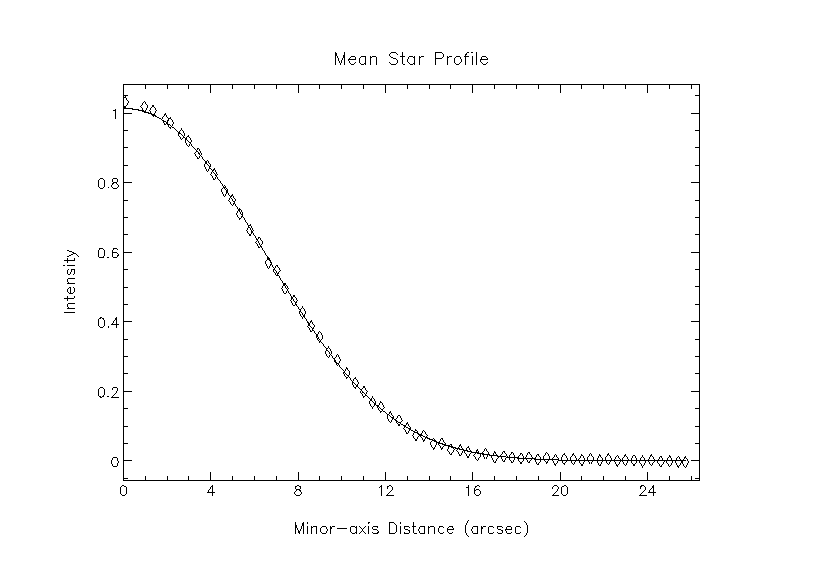
\includegraphics[width=5.5in]{sc11_fig12}
\caption{The radially averaged gaussian fit produced by \psf}
\label{fig:psf}
\end{center}
\end{figure}


This produces the plot shown in Fig.\ \ref{fig:psf}.  The value of FWHM is
14.72'' across the minor axis.  The geometrical mean is simply
$\sqrt{\mbox{mean axis ratio}}$ times 14.72, i.e.\ the measured FWHM
(including the broadening from Uranus) is therefore predicted to be 15.4'' if
we use \psf.  However, if we fit a double Gaussian to the same data set we
obtain 15.56'' $\times$ 14.30'' with a position angle of 85 for the main beam,
and 55.8'' $\times$ 49.6'' for the inner error lobe.  To find the true (HPBW)
we need to remove the broadening caused by Uranus being an extended source.
Using the program \fluxes\ (just type \texttt{fluxes} at the command line and
answer the prompts) we find out that Uranus had a diameter (W) of 3.54'' that
day.  We convert the FWHM measured, $\theta_m$, to the true HPBW of the
telescope, $\theta_{A}$, using the equation \begin{equation} \theta_{A} =
  \sqrt{{\theta_m}^{2} - \frac{ln2}{2} \times W^{2} } \end{equation} where W
the diameter of the planet.  In this case we get 14.5'' for the HPBW and
$\sim$ 53'' for the near (inner) error beam.  If we do the same for 450 $\mu$m
we obtain 7.8'' for the HPBW and 34'' for the near error beam.  These agree
with nominal values for the telescope.


\subsection{\xlabel{calibration_Jy/aperture} Calibrating in Jy/(solid
angle)\label{Calibration_aperture}}

If your maps show simple source morphology and you are only interested
in integrated flux densities, the simplest approach is to calibrate
your map Jy/aperture for the aperture size you want to use.  The
listing of \fluxes\ also gives us the total flux, S$_{tot}$ for Uranus
at 850$\mu$m is 67.9 Jy.  Let us first see how we can use this value
to calibrate our image in terms of Jy/arcsecond$^2$.  In order to do
this we need to derive a value for the Flux Conversion Factor (FCF)
which is in units of Jy/arcsecond$^2$/V. To do this we first need to
work out the sum of the pixel values (V$_{\rm sum}$) in an aperture of
radius r.  We then find the FCF is given by \begin{equation}
FCF(Jy/{\rm arcsecond}^2/V)=67.9/V_{\rm sum}a \end{equation} were a is
the pixel area in square arcseconds.  The easiest way to get the
integrated signal in an aperture is to use \Kappa's \aperadd.  For our
850 $\mu$m map of Uranus we derive V$_{\rm sum}$ for a set of
different circular apertures and compute the FCFs.


\begin{tabular}[c]{llllll}
Radius (arcseconds) & 20 & 30 & 40 & 60 & 120 \\
V$_{\rm sum}$ & 45.75 & 60.76 & 64.89 & 70.07 & 77.08 \\
FCF (Jy/arcsecond$^2$/V) & 1.48 & 1.12 & 1.05 & 0.97 & 0.88 \\
\end{tabular}

We can see from this table that the FCF is dependent on the aperture
size that is used \footnote{During this time period SCUBA had reduced
sensitivity due to a problem in the optics, affecting primarily the
850 $\mu$m array.  Normally you would expect to find a FCF for a 40''
aperture of 0.84, see Jenness et al.\  \cite{Jenness01}} This is
because there is significant signal in the sidelobes and extended
error beam of the telescope.  Clearly then the value of FCF can be
somewhat ambiguous.  What you have to remember is that if you are
doing photometry of an extended object, you should use a value for the
FCF derived for the same aperture.

If you need to use small apertures, i.e.\ the size of your HPBW, you will need
to use a point source or point like source as a calibrator.  Flux densities
for our secondary calibrators for a 40'' aperture are given by Jenness et al.\
\cite{Jenness01}.  However, several of our secondary calibrators are not point
sources.  If you end up with, for example, IRC$+$10216 and IRAS 16293$-$2422
or Mars near perhelion as your only calibrators during your run, you are in
trouble.  You may be able to use a large aperture to recover all the flux and
use the ratios between different apertures derived for a point source.  But,
you may as well bite the bullet and calibrate in {\it Jy/beam}.



\subsection{\xlabel{beam_profiles} Calibrating maps in {\it Jy/beam}
\label{beam}}

If your images show a lot of structure, you will need to calibrate
your maps in {\it Jy/beam}.  This is true for most observations of
dark and molecular clouds, young supernovae, protostars or young stars
and even for nearby galaxies.  However, if you are only dealing with
faint point sources and low S/N maps, you probably need to integrate
over the map.  If this is the case, it does not matter whether you
calibrate in {\it Jy/beam} or {\it Jy/aperture}, both methods will
give the same result.  Since \starlink\ packages do not deal with
Jy/beam, it may appear more complicated to integrate over an image
calibrated in Jy/beam, but the only difference is that one needs to
normalize the integral over the source with the beam integral, $\int
F(\Omega)_\nu d\Omega$, where F($\Omega$) is the normalized power
pattern of the telescope.  For a Gaussian beam the beam integral is
simply $ 1.134 \times \theta_A^2$.  Radio astronomical reduction
packages of course do this normalization automatically.  Since the
JCMT beam is not a simple Gaussian beam, we need to account for the
error beam, which is equivalent to having an FCF which varies with
aperture, when we calibrate in {\it Jy/aperture}.  We discuss how this
is done towards the end of this section.

To calibrate in {\it Jy/beam} we have to know the beam size.  Ideally
we would derive both the flux density conversion factor and the beam
size, $\theta_A$, from planet observations. If there are no planets
available, we can use one of the secondary calibrators. To determine
the beam size at 850 $\mu$m it is usually sufficient to make a weighted
average from our pointing observations during the run, if we don't have
a planet observation or a point like secondary calibrator, but for 450
$\mu$m we need a planet or a secondary calibrator.  All JCMT secondary
calibrators are directly calibrated in {\it Jy/beam}. In this case the
FCF is simply the quoted flux divided by the peak signal of the
source.

\subsubsection{Calibrating on Planets}

For a planet we have to account for the loss of signal due to the
coupling to the beam, because all planets used for calibration are
extended relative to the JCMT beam. For our Uranus data the flux
density S$_{\rm beam}$ is therefore the total flux density, S$_{\rm
tot}$ divided by the coupling of the planet to the beam, given by:
\begin{equation} K = \frac{x^2}{1 - e^{-x^2}} \end{equation} where x
is
\begin{equation} x = \frac{W}{1.2 \times \theta_A}.  \end{equation}

The FCF, in {\it Jy/beam/V} is therefore

\begin{equation} FCF(Jy/{\rm beam}/V) = S_{\rm beam}/V_{\rm peak}
\end{equation}


For 850 $\mu$m we find K = 1.021 for $\theta_A$ = 14.5'', which gives
S$_{beam}$ = 66.5 Jy/beam. The peak signal that we found for our high
S/N Uranus map, V$_{\rm peak}$ = 0.2477 V, or an FCF = 268.5
Jy/beam/V.  This FCF applies to a jiggle maps with a 120'' chop throw.
If we do the same for our jiggle maps of Uranus with a 60'' chop throw,
we derive FCF = 245.2 Jy/beam/V, i.e.\  a map with a 60'' chop throw is
$\sim$ 10\% more efficient than one with a 120'' chop throw. Even
though Jenness et al.\ (\cite{Jenness01}) found no difference in FCF as
a function of chop throw when calibrating in {\it Jy/aperture} we find
that the difference is now smaller than compared to when calibrating in
{\it Jy/beam} but still noticeable. For a 40'' aperture the difference
is 6\%.

\subsubsection{Using secondary calibrators}

If we use a secondary calibrator to calibrate our maps, it is even
simpler. We just take the quoted flux value, S$_{beam}$, from the
secondary calibrator page and divide it with the peak flux in our map
of the same calibrator. If the map of the calibrator has poor S/N, we
may want to fit a gaussian to the source to get a more accurate measure
of the peak signal.

\subsubsection{How do we extract information from a map calibrated in
{\it Jy/beam}}

Analyzing maps calibrated in {\it Jy/beam} is easy; especially if we
want to deduce flux densities for point sources or compact sources even
when the source is embedded in a cloud with strong extended emission.
For a point source the peak flux of the source is the same as the total
flux corrected for any background emission. For an extended source we
need to measure the FWHM and correct it for the measured HPBW of the
telescope. We normally do this by fitting a double Gaussian, one for
the source and one for the background. At 850 $\mu$m the fitted peak
signal minus background, S$_{\rm peak}$, is now the peak flux density
measured in Jy/beam. From the fitted Full Width at Half Maximum (FWHM)
we can derive the true FWHM, $\theta_s$, by deconvolving with the
measured HPBW, $\theta_A$. This is trivial, because now we can assume a
Gaussian source and a Gaussian beam. After we know the source size,
$\theta_s$ we multiply the peak flux with the correction factor we
derive from the size, i.e.\ for a spherically symmetric source with the
source size,  $\theta_{s}$, the total flux, S$_{\rm tot}$ is simply

\begin{equation}
S_{\rm tot} = S_{\rm peak} \times (1 +(\theta_{s}/\theta_{A})^2)   \end{equation}.

For 450 $\mu$m the error beam amplitude is no longer negligible, but
when we fit a double Gaussian, the error beam will blend in with the
extended cloud emission, i.e.\ it adds into the background level, or we
may fit the source with a single Gaussian plus a second order surface,
or whatever best approximates the background in a limited area around
the source.  From our analysis of the 450 $\mu$m beam maps of Uranus,
we find that the combined error beam amplitude is of the order of 5\%
of the peak amplitude, and we should therefore multiply the peak
signal by 1.05 before applying a source size correction (see e.g.\
Weintraub et al.\  \cite{Weintraub99}).


To find integrated intensities over large areas is more complicated,
because now we need to correct for the error beam pickup, which now
depends on the area we integrate over.  This is equivalent to the
varying the FCF as a function of aperture that one has to account for
if the map is calibrated in {\it Jy/pixel}, but with the map
calibrated in {\it Jy/beam} it is much easier to separate compact
sources and extended emission.  To determine the excess emission from
the error beam, we again have to go back to our beam map.  If we
calibrate our 850 $\mu$m map in Jy/beam and then integrate over 120''
circular aperture, we find that the flux we derive is 86.8 Jy, while
we know that the total flux of Uranus is only 67.9 Jy.  We therefore
have to scale our derived total flux density by the ratio of true flux
density over measured flux density (for our calibrated planet map),
which in this case is 0.78.  At 450 $\mu$m the situation is much
worse.  Even though the amplitude of the error lobe is still low, the
area is large, and if we integrate over our calibrated 450 $\mu$m beam
map we now derive 415.6 Jy, if we integrate over the same 120"
circular aperture, while the total flux density from \fluxes\ is only
179.3 Jy.  In this case our scaling factor is 0.43, i.e.\ we pick up
more emission in the extended error beam than we do in the main beam.

For careful work, you may therefore want to deconvolve your SCUBA
maps.  This becomes especially important if you want to ratio the 450
and the 850 $\mu$m maps, because if you want to smooth the 450 $\mu$m
map to the same resolution as the 850 $\mu$m map, you first have to
remove the error beam.  For example of how this can be done, see e.g.\
Hogherheijde and Sandell \cite{Hogherheijde00} or Sandell and
Weintraub \cite{Sandell01}.

\clearpage

\section{\xlabel{common_error-messages_--_what_have_i_done_wrong}Common error-messages -- what have I done wrong?}

\begin{description}

\item[The computer does not find the command task]\mbox{}

You probably have forgotten to initialize \surf\ or \Kappa.

\item[The computer does not recognize the command SURF]\mbox{}

Let's assume that you have followed the manual, and you type
\texttt{surf}
to initialize the \surf\ software package, but nothing happens.  You
get
a reply saying command not found, instead of the listing you saw in
the
manual. In this case you probably lack the \starlink\ initialization
in
your \texttt{.cshrc} and \texttt{.login} files. Type

\begin{myquote} \begin{verbatim}
% source /star/etc/login
% source /star/etc/cshrc
\end{verbatim} \end{myquote}

and you should be able to initialize \surf\ and \Kappa. The \starlink\
initialization scripts should be placed in your \texttt{.cshrc} and
\texttt{.login} files if you intend to use \surf\ and \Kappa\
regularly:

i.e.\ in your \texttt{.login} file put the line:
\begin{myquote}
\begin{verbatim}
if (-e /star/etc/login) source /star/etc/login
\end{verbatim}
\end{myquote}
and in  your \texttt{.cshrc} file put the line:
\begin{myquote}
\begin{verbatim}
if (-e /star/etc/cshrc) source /star/etc/cshrc
\end{verbatim}
\end{myquote}

See, for example, \xref{SUN/212}{sun212}{} \cite{sun212}  for more
information on using and installing \starlink\ software.

\item[KAPPA tasks like \task{centroid} pick up the wrong image]\mbox{}

This seems to occasionally happen when we switch between program
packages. The cure is to delete the \agi\ \cite{agi} resource file,
called \texttt{agi\_computer.sdf}, where \texttt{computer} is the name
of your computer, and the file resides in your home directory. In my
case the file is called \texttt{/home/sandell/kala\_agi.sdf}.

\item[KAPPA \task{display} plots a new image inside an old
image]\mbox{}

This means that your \agi\ database has become corrupt (e.g.\ by using
control-C to exit early from a task that displays graphics (\scuover\
for
example) -- this prevents the task from performing normal cleanup
duties). This problem can be fixed by issuing the \Kappa\ command
\gdclear\ or
by removing the \agi\ database file from your home directory (see
earlier
fault).

\item[I get a grayscale hardcopy, even though I specified a color
device]\mbox{}

Any color printer will need the color table supplied with the plot. In
addition to setting the device to a color printer (e.g.\ epsfcol\_p),
you will
also have to specify the color table with the parameter \param{lut}.
In the
example below we plot the final NGC\,7129 image using the bgyrw color
table,
which resides in \$KAPPA\_DIR as bgyrw\_lut

\begin{myquote} \begin{verbatim}
% display axes clear n7129_lon lut=$KAPPA_DIR/bgyrw device=epsfcol_p \
    mode=scale
\end{verbatim} \end{myquote}

This produces a color postscript file gks74.ps.n. A list of valid
devices
can be obtained with the \Kappa\ command \gdnames.


\item[Cannot create data array ...]\mbox{}

Error messages of this type typically indicate that you are out of
disk space -- a quite common occurrence for anybody reducing SCUBA
maps --
or that you do not have write permission in your current directory.

\end{description}

\begin{thebibliography}{}
\addcontentsline{toc}{section}{References}

\bibitem{agi}
 Eaton~N., McIlwrath,~B., 2000, \textit{AGI--Applications Graphics
Interface Library}
\xref{AGI}{sun48}{}

\bibitem{surf}
Jenness~T., Lightfoot~J.~F., 1997, \textit{SURF -- SCUBA User
Reduction Facility},
\xref{Starlink User Note 216}{sun216}{} (see also the SURF homepage:
\htmladdnormallink{http://www.jach.hawaii.edu/jcmt\_sw/scuba/surf/}{http://www.jach.hawaii.edu/jcmt_sw/scuba/surf/})


\bibitem{sun212}
Bly~M.~J., 2000, {\it Starlink  Software CD-ROMs Spring 2000 User's
Guide}
\xref{Starlink  Software CD-ROMs Spring 2000 User's Guide}{sun212}{}


\bibitem{kappa}
Currie~M.~J., 1997, {\it KAPPA --- Kernel Application Package},
\xref{Starlink User Note 95}{sun95}{}

\bibitem{figaro}
Shortridge~K., Meyerdierks~H., Currie~M.~J., Clayton~M.,
{\it FIGARO -- A general data reduction system},
\xref{Starlink User Note 86}{sun86}{}

\bibitem{gaia}
Draper~P.~W., 1997, {\it GAIA -- Graphical Astronomy and Image
Analysis Tool},
\xref{Starlink User Note 214}{sun214}{}


\bibitem{jcmtdr}
Lightfoot~J.~F., Harrison~P.~A., Meyerdierks~H., 1995, \textit{JCMTDR
-- Applications for reducing JCMT data}, \xref{Starlink User Note
132}{sun132}{}


\bibitem{skydip}
Duncan,~W.~D., SCUBA project documentation, SCU/WDD/31.1/1093

\bibitem{nod2}
Emerson, D.T., Klein, U., \& Haslam, C.G.T., 1979, A\&A, 76, 92

\bibitem{convert}
Currie~M.~J., Privett~G.~J., Chipperfield~A.~J., 1995 {\it CONVERT --
A format-conversion package}, \xref{Starlink User Note 55}{sun55}{}

\bibitem{Archibald00}
Archibald, E., Wagg, J., Jenness, T, 2000 {Calculating Sky Opacities:
a
re-analysis for SCUBA data},
{\htmladdnormallink{http://www.jach.hawaii.edu/JACdocs/JCMT/SCD/SN/002.2/}{http://www.jach.hawaii.edu/JACdocs/JCMT/SCD/SN/002.2/

} }

\bibitem{Coulson}
Coulson, I., 2001 { Scuba Jiggle Maps},
{\htmladdnormallink{http://www.jach.hawaii.edu/JACdocs/JCMT/SCD/SN/003}{http://www.jach.hawaii.edu/JACdocs/JCMT/SCD/SN/003}}

\bibitem{Hogherheijde00}
Hogherheijde, M.R., Sandell, G., 2000, ApJ, 534, 880

\bibitem{Jenness01}
Jenness, T., Stevens, J.A., Archibald, E.N., Economou, F., Jessop,
N.E., Robson, E.I., 2001, MNRAS, submitted

\bibitem{Pierce00}
Pierce-Price, D., et al., 2000, ApJ, 545, L121

\bibitem{Sandell01}
Sandell, G., Weintraub, D.A., 2001, ApJS, 134, 115

\bibitem{Weintraub99}
Weintraub, D.A., et al., 1999, ApJ, 517, 819


\end{thebibliography}

\end{document}



%%% Local Variables:
%%% mode: latex
%%% TeX-master: "sc11"
%%% End:
